\PassOptionsToPackage{unicode=true}{hyperref} % options for packages loaded elsewhere
\PassOptionsToPackage{hyphens}{url}
%
\documentclass[a4paperpaper,openright]{book}
\usepackage{lmodern}
\usepackage{amssymb,amsmath}
\usepackage{ifxetex,ifluatex}
\usepackage{fixltx2e} % provides \textsubscript
\ifnum 0\ifxetex 1\fi\ifluatex 1\fi=0 % if pdftex
  \usepackage[T1]{fontenc}
  \usepackage[utf8]{inputenc}
  \usepackage{textcomp} % provides euro and other symbols
\else % if luatex or xelatex
  \usepackage{unicode-math}
  \defaultfontfeatures{Ligatures=TeX,Scale=MatchLowercase}
\fi
% use upquote if available, for straight quotes in verbatim environments
\IfFileExists{upquote.sty}{\usepackage{upquote}}{}
% use microtype if available
\IfFileExists{microtype.sty}{%
\usepackage[]{microtype}
\UseMicrotypeSet[protrusion]{basicmath} % disable protrusion for tt fonts
}{}
\IfFileExists{parskip.sty}{%
\usepackage{parskip}
}{% else
\setlength{\parindent}{0pt}
\setlength{\parskip}{6pt plus 2pt minus 1pt}
}
\usepackage{hyperref}
\hypersetup{
            pdfborder={0 0 0},
            breaklinks=true}
\urlstyle{same}  % don't use monospace font for urls
\usepackage{color}
\usepackage{fancyvrb}
\newcommand{\VerbBar}{|}
\newcommand{\VERB}{\Verb[commandchars=\\\{\}]}
\DefineVerbatimEnvironment{Highlighting}{Verbatim}{commandchars=\\\{\}}
% Add ',fontsize=\small' for more characters per line
\newenvironment{Shaded}{}{}
\newcommand{\AlertTok}[1]{\textcolor[rgb]{1.00,0.00,0.00}{\textbf{#1}}}
\newcommand{\AnnotationTok}[1]{\textcolor[rgb]{0.38,0.63,0.69}{\textbf{\textit{#1}}}}
\newcommand{\AttributeTok}[1]{\textcolor[rgb]{0.49,0.56,0.16}{#1}}
\newcommand{\BaseNTok}[1]{\textcolor[rgb]{0.25,0.63,0.44}{#1}}
\newcommand{\BuiltInTok}[1]{#1}
\newcommand{\CharTok}[1]{\textcolor[rgb]{0.25,0.44,0.63}{#1}}
\newcommand{\CommentTok}[1]{\textcolor[rgb]{0.38,0.63,0.69}{\textit{#1}}}
\newcommand{\CommentVarTok}[1]{\textcolor[rgb]{0.38,0.63,0.69}{\textbf{\textit{#1}}}}
\newcommand{\ConstantTok}[1]{\textcolor[rgb]{0.53,0.00,0.00}{#1}}
\newcommand{\ControlFlowTok}[1]{\textcolor[rgb]{0.00,0.44,0.13}{\textbf{#1}}}
\newcommand{\DataTypeTok}[1]{\textcolor[rgb]{0.56,0.13,0.00}{#1}}
\newcommand{\DecValTok}[1]{\textcolor[rgb]{0.25,0.63,0.44}{#1}}
\newcommand{\DocumentationTok}[1]{\textcolor[rgb]{0.73,0.13,0.13}{\textit{#1}}}
\newcommand{\ErrorTok}[1]{\textcolor[rgb]{1.00,0.00,0.00}{\textbf{#1}}}
\newcommand{\ExtensionTok}[1]{#1}
\newcommand{\FloatTok}[1]{\textcolor[rgb]{0.25,0.63,0.44}{#1}}
\newcommand{\FunctionTok}[1]{\textcolor[rgb]{0.02,0.16,0.49}{#1}}
\newcommand{\ImportTok}[1]{#1}
\newcommand{\InformationTok}[1]{\textcolor[rgb]{0.38,0.63,0.69}{\textbf{\textit{#1}}}}
\newcommand{\KeywordTok}[1]{\textcolor[rgb]{0.00,0.44,0.13}{\textbf{#1}}}
\newcommand{\NormalTok}[1]{#1}
\newcommand{\OperatorTok}[1]{\textcolor[rgb]{0.40,0.40,0.40}{#1}}
\newcommand{\OtherTok}[1]{\textcolor[rgb]{0.00,0.44,0.13}{#1}}
\newcommand{\PreprocessorTok}[1]{\textcolor[rgb]{0.74,0.48,0.00}{#1}}
\newcommand{\RegionMarkerTok}[1]{#1}
\newcommand{\SpecialCharTok}[1]{\textcolor[rgb]{0.25,0.44,0.63}{#1}}
\newcommand{\SpecialStringTok}[1]{\textcolor[rgb]{0.73,0.40,0.53}{#1}}
\newcommand{\StringTok}[1]{\textcolor[rgb]{0.25,0.44,0.63}{#1}}
\newcommand{\VariableTok}[1]{\textcolor[rgb]{0.10,0.09,0.49}{#1}}
\newcommand{\VerbatimStringTok}[1]{\textcolor[rgb]{0.25,0.44,0.63}{#1}}
\newcommand{\WarningTok}[1]{\textcolor[rgb]{0.38,0.63,0.69}{\textbf{\textit{#1}}}}
\usepackage{graphicx,grffile}
\makeatletter
\def\maxwidth{\ifdim\Gin@nat@width>\linewidth\linewidth\else\Gin@nat@width\fi}
\def\maxheight{\ifdim\Gin@nat@height>\textheight\textheight\else\Gin@nat@height\fi}
\makeatother
% Scale images if necessary, so that they will not overflow the page
% margins by default, and it is still possible to overwrite the defaults
% using explicit options in \includegraphics[width, height, ...]{}
\setkeys{Gin}{width=\maxwidth,height=\maxheight,keepaspectratio}
\setlength{\emergencystretch}{3em}  % prevent overfull lines
\providecommand{\tightlist}{%
  \setlength{\itemsep}{0pt}\setlength{\parskip}{0pt}}
\setcounter{secnumdepth}{0}
% Redefines (sub)paragraphs to behave more like sections
\ifx\paragraph\undefined\else
\let\oldparagraph\paragraph
\renewcommand{\paragraph}[1]{\oldparagraph{#1}\mbox{}}
\fi
\ifx\subparagraph\undefined\else
\let\oldsubparagraph\subparagraph
\renewcommand{\subparagraph}[1]{\oldsubparagraph{#1}\mbox{}}
\fi

% set default figure placement to htbp
\makeatletter
\def\fps@figure{htbp}
\makeatother

% Table of contents formatting
\renewcommand{\contentsname}{Table of Contents}
\setcounter{tocdepth}{3}

\setcounter{secnumdepth}{4}


% \renewcommand\thesection{\Roman{section}}

 
% Headers and page numbering 
\usepackage{fancyhdr}

\fancyhead{}
\fancyhead[R]{\leftmark}
\renewcommand{\headrulewidth}{0.4pt}

\fancyfoot[R]{\thepage}
\fancyfoot[C]{}
\fancyfoot[L]{\textit{An Introduction to Symfony 6 \copyright Matt Smith 2022}}
\renewcommand{\footrulewidth}{0.4pt}

\pagestyle{fancy}

% Fonts and typesetting
\setsansfont{Verdana}

% Set figure legends and captions to be smaller sized sans serif font
\usepackage[font={footnotesize,sf}]{caption}

\usepackage{siunitx}

% Adjust spacing between lines to 1.5
\usepackage{setspace}
\onehalfspacing
\raggedbottom

% Set margins
\usepackage[top=1.25in,bottom=1.25in]{geometry}

% Chapter styling
\usepackage[grey]{quotchap}
\makeatletter
\renewcommand*{\chapnumfont}{%
  \usefont{T1}{\@defaultcnfont}{b}{n}\fontsize{80}{100}\selectfont% Default: 100/130
  \color{chaptergrey}%
}
\makeatother

% Set colour of links to black so that they don't show up when printed
\usepackage{hyperref}
\hypersetup{colorlinks=true, linkcolor=black}

% Tables
\usepackage{booktabs}
\usepackage{threeparttable}
\usepackage{array}
\newcolumntype{x}[1]{%
>{\centering\arraybackslash}m{#1}}%

% Allow for long captions and float captions on opposite page of figures 
\usepackage[rightFloats, CaptionBefore]{fltpage}

% Don't let floats cross subsections
\usepackage[section,subsection]{extraplaceins}

\date{}

\begin{document}

\begin{titlepage}
    \begin{center}
    
        \vspace*{1cm}
        

       \large{ \textbf{ \uppercase{An Introduction to Symfony 6}\\(for people that already know OO-PHP and some MVC stuff)}}
        
        \vspace{1.5cm}

        by\\
        \textbf{
        Matt Smith, Ph.D.\\https://github.com/dr-matt-smith
        }

       

        
        
        \vfill
  
            \copyright ~ 2022

     \end{center}
    \thispagestyle{empty}
\end{titlepage}

\newpage
\thispagestyle{empty}
\mbox{}

\frontmatter

\chapter{Acknowledgements}

Thanks to Ryan Weaver, for suggesting I update things to Symfony 6 in
2022 :-)

Thanks to the PHP and Symfony open-source international communities.

\tableofcontents

\mainmatter

\part{Symfony Testing}

\hypertarget{unit-testing-in-symfony}{%
\chapter{Unit testing in Symfony}\label{unit-testing-in-symfony}}

\hypertarget{testing-in-symfony}{%
\section{Testing in Symfony}\label{testing-in-symfony}}

Symfony is built by an open source community. There is a lot of
information about how to test Symfony in the official documentation
pages:

\begin{itemize}
\item
  \href{http://symfony.com/doc/current/testing.html}{Symfony testing}
\item
  \href{http://symfony.com/doc/current/testing/simulating_authentication.html}{Testing
  with user authentication tokens}
\item
  \href{http://symfony.com/doc/current/testing/http_authentication.html}{How
  to Simulate HTTP Authentication in a Functional Test}
\end{itemize}

\hypertarget{installing-simple-phpunit-project-test01}{%
\section{\texorpdfstring{Installing Simple-PHPUnit (project
\texttt{test01})}{Installing Simple-PHPUnit (project test01)}}\label{installing-simple-phpunit-project-test01}}

Symfony has as special `testpack' that works with PHPUnit. Add this to
your project as follows:

\begin{Shaded}
\begin{Highlighting}[]
\NormalTok{    $ }\ExtensionTok{composer}\NormalTok{ require --dev symfony/test-pack}
\end{Highlighting}
\end{Shaded}

You should now see a \texttt{/tests} directory created.

Run our tests - we have none, so should get a message telling us no
tests were executed:

\begin{Shaded}
\begin{Highlighting}[]
\NormalTok{    $ }\ExtensionTok{bin/phpunit}

    \ExtensionTok{PHPUnit}\NormalTok{ 9.5.19}

    \ExtensionTok{No}\NormalTok{ tests executed!}
\end{Highlighting}
\end{Shaded}

\hypertarget{creating-a-test-class}{%
\section{Creating a test class}\label{creating-a-test-class}}

Let's create a simple test (1 + 1 = 2!) to check everything is working
okay.

Create a new class \texttt{/tests/SimpleTest.php} containing the
following:

\begin{Shaded}
\begin{Highlighting}[]
\NormalTok{    <}\OtherTok{?}\NormalTok{php}
    \KeywordTok{namespace}\NormalTok{ App\textbackslash{}Tests}\OtherTok{;}

    \KeywordTok{use}\NormalTok{ PHPUnit\textbackslash{}Framework\textbackslash{}TestCase}\OtherTok{;}

    \KeywordTok{class}\NormalTok{ SimpleTest }\KeywordTok{extends}\NormalTok{ TestCase}
\NormalTok{    \{}
        \KeywordTok{public} \KeywordTok{function}\NormalTok{ testOnePlusOneEqualsTwo}\OtherTok{()}
\NormalTok{        \{}
            \CommentTok{// Arrange}
            \KeywordTok{$num1}\NormalTok{ = }\DecValTok{1}\OtherTok{;}
            \KeywordTok{$num2}\NormalTok{ = }\DecValTok{1}\OtherTok{;}
            \KeywordTok{$expectedResult}\NormalTok{ = }\DecValTok{2}\OtherTok{;}

            \CommentTok{// Act}
            \KeywordTok{$result}\NormalTok{ = }\KeywordTok{$num1}\NormalTok{ + }\KeywordTok{$num2}\OtherTok{;}

            \CommentTok{// Assert}
            \KeywordTok{$this}\NormalTok{->assertEquals}\OtherTok{(}\KeywordTok{$expectedResult}\OtherTok{,} \KeywordTok{$result}\OtherTok{);}
\NormalTok{        \}}
\NormalTok{    \}}
\end{Highlighting}
\end{Shaded}

Note the following:

\begin{itemize}
\item
  test classes are located in directory \texttt{/tests}

  \begin{itemize}
  \tightlist
  \item
    or a suitably named sub-directory, matching the \texttt{/src}
    namespaced folder they are testing
  \end{itemize}
\item
  test classes end with the suffix \texttt{Test},
  e.g.~\texttt{SimpleTest}
\item
  simple test classes extend the superclass
  \texttt{\textbackslash{}PHPUnit\textbackslash{}Framework\textbackslash{}TestCase}

  -- if we add a \texttt{uses} statement
  \texttt{use\ PHPUnit\textbackslash{}Framework\textbackslash{}TestCase}
  then we can simple extend \texttt{TestCase}
\item
  simple test classes are in namespace \texttt{App\textbackslash{}Tests}

  -- the names and namespaces of test classes testing a class in
  \texttt{/src} will reflect the namespace of the class being tested

  -- i.e.~If we write a class to test
  \texttt{/src/Controller/DefaultController.php} it will be
  \texttt{/tests/Controller/DefaultControllerTest.php}, and it will be
  in namespace
  \texttt{App\textbackslash{}Tests\textbackslash{}Controller}

  -- so our testing class architecture directly matches our source code
  architecture
\end{itemize}

\hypertarget{running-our-tests}{%
\section{Running our tests}\label{running-our-tests}}

Run our tests - we have 1 now, so should get a message telling us our
test ran and passed:

\begin{Shaded}
\begin{Highlighting}[]
\NormalTok{    $ }\ExtensionTok{bin/phpunit}

    \ExtensionTok{Testing}
    \BuiltInTok{.}                                                                   \ExtensionTok{1}\NormalTok{ / 1 (100%)}

    \ExtensionTok{Time}\NormalTok{: 00:00.022, Memory: 10.00 MB}

    \ExtensionTok{OK}\NormalTok{ (1 test, 1 assertion)}
\end{Highlighting}
\end{Shaded}

Dots are good. For each passed test you'll see a full stop. Then after
all tests have run, you'll see a summary:

\begin{Shaded}
\begin{Highlighting}[]
    \ExtensionTok{1}\NormalTok{ / 1 (100%)}
\end{Highlighting}
\end{Shaded}

This tells us how many passed, out of how many, and what the pass
percentage was. In our case, 1 out of 1 passed = 100\%.

\hypertarget{testing-other-classes-project-test02}{%
\section{\texorpdfstring{Testing other classes (project
\texttt{test02})}{Testing other classes (project test02)}}\label{testing-other-classes-project-test02}}

\textbf{our testing structure mirrors the code we are testing}

Let's create a very simple class \texttt{Calculator.php} in
\texttt{/src/Util}\footnote{Short for `Utility' - i.e.~useful stuff!},
and then write a class to test our class. Our simple class will be a
very simple calculator:

\begin{itemize}
\item
  method \texttt{add(...)} accepts 2 numbers and returns the result of
  adding them
\item
  method \texttt{subtract()} accepts 2 numbers and returns the result of
  subtracting the second from the first
\end{itemize}

so our \texttt{Calculator} class is as follows:

\begin{Shaded}
\begin{Highlighting}[]
\NormalTok{    <}\OtherTok{?}\NormalTok{php}
    \KeywordTok{namespace}\NormalTok{ App\textbackslash{}Util}\OtherTok{;}

    \KeywordTok{class}\NormalTok{ Calculator}
\NormalTok{    \{}
        \KeywordTok{public} \KeywordTok{function}\NormalTok{ add}\OtherTok{(}\KeywordTok{$n1}\OtherTok{,} \KeywordTok{$n2}\OtherTok{)}
\NormalTok{        \{}
            \KeywordTok{return} \KeywordTok{$n1}\NormalTok{ + }\KeywordTok{$n2}\OtherTok{;}
\NormalTok{        \}}

        \KeywordTok{public} \KeywordTok{function}\NormalTok{ subtract}\OtherTok{(}\KeywordTok{$n1}\OtherTok{,} \KeywordTok{$n2}\OtherTok{)}
\NormalTok{        \{}
            \KeywordTok{return} \KeywordTok{$n1}\NormalTok{ - }\KeywordTok{$n2}\OtherTok{;}
\NormalTok{        \}}
\NormalTok{    \}}
\end{Highlighting}
\end{Shaded}

\hypertarget{the-class-to-test-our-calculator}{%
\section{The class to test our
calculator}\label{the-class-to-test-our-calculator}}

We now need to write a test class to test our calculator class. Since
our source code class is \texttt{/src/Util/Calculator.php} then our
testing class will be \texttt{/tests/Util/CalculatorTest.php}. And since
the namespace of our source code class was
\texttt{App\textbackslash{}Util} then the namespace of our testing class
will be \texttt{App\textbackslash{}Tests\textbackslash{}Util}. Let's
test making an instance-object of our class \texttt{Calculator}, and we
will make 2 assertions:

\begin{itemize}
\item
  the reference to the new object is not NULL
\item
  invoking the \texttt{add(...)} method with arguments of (1,1) and
  returns the correct answer (2!)
\end{itemize}

Here's the listing for our new test class
\texttt{/tests/Util/CalculatorTest.php}:

\begin{Shaded}
\begin{Highlighting}[]
    \KeywordTok{namespace}\NormalTok{ App\textbackslash{}Tests\textbackslash{}Util}\OtherTok{;}

    \KeywordTok{use}\NormalTok{ App\textbackslash{}Util\textbackslash{}Calculator}\OtherTok{;}
    \KeywordTok{use}\NormalTok{ PHPUnit\textbackslash{}Framework\textbackslash{}TestCase}\OtherTok{;}

    \KeywordTok{class}\NormalTok{ CalculatorTest }\KeywordTok{extends}\NormalTok{ TestCase}
\NormalTok{    \{}
        \KeywordTok{public} \KeywordTok{function}\NormalTok{ testCanCreateObject}\OtherTok{()}
\NormalTok{        \{}
            \CommentTok{// Arrange}
            \KeywordTok{$calculator}\NormalTok{ = }\KeywordTok{new}\NormalTok{ Calculator}\OtherTok{();}

            \CommentTok{// Act}

            \CommentTok{// Assert}
            \KeywordTok{$this}\NormalTok{->assertNotNull}\OtherTok{(}\KeywordTok{$calculator}\OtherTok{);}
\NormalTok{        \}}

        \KeywordTok{public} \KeywordTok{function}\NormalTok{ testAddOneAndOne}\OtherTok{()}
\NormalTok{        \{}
            \CommentTok{// Arrange}
            \KeywordTok{$calculator}\NormalTok{ = }\KeywordTok{new}\NormalTok{ Calculator}\OtherTok{();}
            \KeywordTok{$num1}\NormalTok{ = }\DecValTok{1}\OtherTok{;}
            \KeywordTok{$num2}\NormalTok{ = }\DecValTok{1}\OtherTok{;}
            \KeywordTok{$expectedResult}\NormalTok{ = }\DecValTok{2}\OtherTok{;}

            \CommentTok{// Act}
            \KeywordTok{$result}\NormalTok{ = }\KeywordTok{$calculator}\NormalTok{->add}\OtherTok{(}\KeywordTok{$num1}\OtherTok{,} \KeywordTok{$num2}\OtherTok{);}

            \CommentTok{// Assert}
            \KeywordTok{$this}\NormalTok{->assertEquals}\OtherTok{(}\KeywordTok{$expectedResult}\OtherTok{,} \KeywordTok{$result}\OtherTok{);}
\NormalTok{        \}}
\NormalTok{    \}}
\end{Highlighting}
\end{Shaded}

Note:

\begin{itemize}
\tightlist
\item
  we had to add \texttt{use} statements for the class we are testing
  (\texttt{App\textbackslash{}Util\textbackslash{}Calculator}) and the
  PHP Unit TestCase class we are extending
  (\texttt{use\ PHPUnit\textbackslash{}Framework\textbackslash{}TestCase})
\end{itemize}

Run the tests - if all goes well we should see 3 out of 3 tests passing:

\begin{Shaded}
\begin{Highlighting}[]
\NormalTok{    $ }\ExtensionTok{bin/phpunit}

    \ExtensionTok{Testing}
    \ExtensionTok{...}\NormalTok{                                                                 3 / 3 (100%)}

    \ExtensionTok{Time}\NormalTok{: 00:00.014, Memory: 10.00 MB}

    \ExtensionTok{OK}\NormalTok{ (3 tests, 3 assertions)}
\end{Highlighting}
\end{Shaded}

\hypertarget{using-a-data-provider-to-test-with-multiple-datasets}{%
\section{Using a data provider to test with multiple
datasets}\label{using-a-data-provider-to-test-with-multiple-datasets}}

Rather than writing lots of methods to test different additions, let's
use a \textbf{data provider} (via an annotation comment), to provide a
single method with many sets of input and expected output values:

Here is our testing method:

\begin{Shaded}
\begin{Highlighting}[]
    \CommentTok{/**}
\CommentTok{     * }\AnnotationTok{@dataProvider}\CommentTok{ additionProvider}
\CommentTok{     */}
    \KeywordTok{public} \KeywordTok{function}\NormalTok{ testAdditionsWithProvider}\OtherTok{(}\KeywordTok{$num1}\OtherTok{,} \KeywordTok{$num2}\OtherTok{,} \KeywordTok{$expectedResult}\OtherTok{)}
\NormalTok{    \{}
        \CommentTok{// Arrange}
        \KeywordTok{$calculator}\NormalTok{ = }\KeywordTok{new}\NormalTok{ Calculator}\OtherTok{();}

        \CommentTok{// Act}
        \KeywordTok{$result}\NormalTok{ = }\KeywordTok{$calculator}\NormalTok{->add}\OtherTok{(}\KeywordTok{$num1}\OtherTok{,} \KeywordTok{$num2}\OtherTok{);}

        \CommentTok{// Assert}
        \KeywordTok{$this}\NormalTok{->assertEquals}\OtherTok{(}\KeywordTok{$expectedResult}\OtherTok{,} \KeywordTok{$result}\OtherTok{);}
\NormalTok{    \}}
\end{Highlighting}
\end{Shaded}

and here is the data provider (an array of arrays, with the right number
of values for the parameters of \texttt{testAdditionsWithProvider(...)}:

\begin{Shaded}
\begin{Highlighting}[]
    \KeywordTok{public} \KeywordTok{function}\NormalTok{ additionProvider}\OtherTok{()}
\NormalTok{    \{}
        \KeywordTok{return} \OtherTok{[}
            \OtherTok{[}\DecValTok{1}\OtherTok{,} \DecValTok{1}\OtherTok{,} \DecValTok{2}\OtherTok{],}
            \OtherTok{[}\DecValTok{2}\OtherTok{,} \DecValTok{2}\OtherTok{,} \DecValTok{4}\OtherTok{],}
            \OtherTok{[}\DecValTok{0}\OtherTok{,} \DecValTok{1}\OtherTok{,} \DecValTok{1}\OtherTok{],}
        \OtherTok{];}
\NormalTok{    \}}
\end{Highlighting}
\end{Shaded}

Take special note of the annotation comment immediately before method
\texttt{testAdditionsWithProvider(...)}:

\begin{Shaded}
\begin{Highlighting}[]
    \CommentTok{/**}
\CommentTok{     * }\AnnotationTok{@dataProvider}\CommentTok{ additionProvider}
\CommentTok{     */}
\end{Highlighting}
\end{Shaded}

The special comment starts with \texttt{/**}, and declares an annotation
\texttt{@dataProvider}, followed by the name (identifier) of the method.
Note especially that there are no parentheses \texttt{()} after the
method name.

When we run Simple-PHPUnit now we see lots of tests being executed,
repeatedly invoking \texttt{testAdditionsWithProvider(...)} with
different arguments from the provider:

\begin{Shaded}
\begin{Highlighting}[]
\NormalTok{    $ }\ExtensionTok{vendor/bin/simple-phpunit}
    \ExtensionTok{PHPUnit}\NormalTok{ 5.7.27 by Sebastian Bergmann and contributors.}

    \ExtensionTok{Testing}\NormalTok{ Project Test Suite}
    \ExtensionTok{......}\NormalTok{                                                              6 / 6 (100%)}

    \ExtensionTok{Time}\NormalTok{: 65 ms, Memory: 4.00MB}

    \ExtensionTok{OK}\NormalTok{ (6 tests, 6 assertions)}
\end{Highlighting}
\end{Shaded}

\hypertarget{configuring-testing-reports}{%
\section{Configuring testing
reports}\label{configuring-testing-reports}}

In additional to instant reporting at the command line, PHPUnit offers
several different methods of recording test output text-based files.

PHPUnit (when run with Symfony's Simple-PHPUnit) reads configuration
settings from file \texttt{phpunit.dist.xml}. Most of the contents of
this file (created as part of the installation of the Simple-PHPUnit
package) can be left as their defaults. But we can add a range of logs
by adding the following `logging' element in this file.

Many projects follow a convention where testing output files are stored
in a directory named \texttt{build}. We'll follow that convention below
- but of course change the name and location of the test logs to
anywhere you want.

Add the following into file \texttt{phpunit.dist.xml}:

\begin{Shaded}
\begin{Highlighting}[]
    \KeywordTok{<logging>}
        \KeywordTok{<junit}\OtherTok{ outputFile=}\StringTok{"junit.xml"}\KeywordTok{/>}
        \KeywordTok{<teamcity}\OtherTok{ outputFile=}\StringTok{"./build/teamcity.txt"}\KeywordTok{/>}
        \KeywordTok{<testdoxHtml}\OtherTok{ outputFile=}\StringTok{"./build/testdox.html"}\KeywordTok{/>}
        \KeywordTok{<testdoxText}\OtherTok{ outputFile=}\StringTok{"./build/testdox.txt"}\KeywordTok{/>}
        \KeywordTok{<testdoxXml}\OtherTok{ outputFile=}\StringTok{"./build/testdox.xml"}\KeywordTok{/>}
        \KeywordTok{<text}\OtherTok{ outputFile=}\StringTok{"./build/logfile.txt"}\KeywordTok{/>}
    \KeywordTok{</logging>}
\end{Highlighting}
\end{Shaded}

Figure \ref{build_contents} shows a screenshot of the contents of the
created \texttt{/build} directory after Simple-PHPUnit has been run.

\begin{figure}
\centering
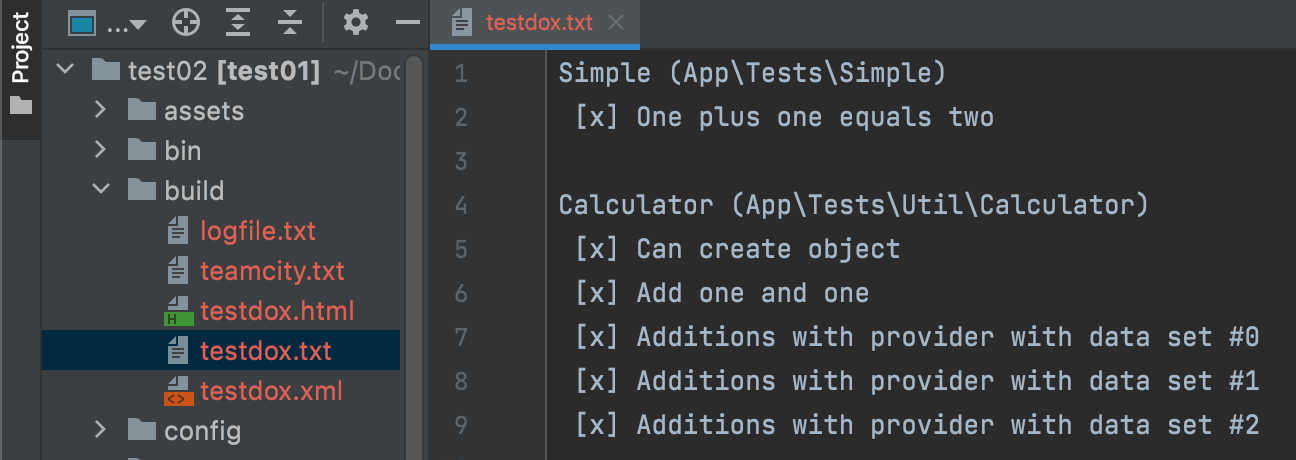
\includegraphics{./tex2pdf.-05a85d9d563be472/3559f32c2528365c9a16e82840e354027eaf070d.png}
\caption{Contents of directory \texttt{/build}. \label{build_contents}}
\end{figure}

The \texttt{.txt} file version of \textbf{test dox}
(\textbf{testdoxText}) is perhaps the simplest output - showing
\texttt{{[}x{]}} next to a passed method and \texttt{{[}\ {]}} for a
test that didn't pass. The text output turns the test method names into
more English-like sentences:

\begin{verbatim}
     Simple (App\Tests\Simple)
      [x] One plus one equals two

     Calculator (App\Tests\Util\Calculator)
      [x] Can create object
      [x] Add one and one
      [x] Additions with provider with data set #0
      [x] Additions with provider with data set #1
      [x] Additions with provider with data set #2
\end{verbatim}

\hypertarget{testing-for-exceptions-project-test03}{%
\section{\texorpdfstring{Testing for exceptions (project
\texttt{test03})}{Testing for exceptions (project test03)}}\label{testing-for-exceptions-project-test03}}

If our code throws an \textbf{Exception} while a test is being executed,
and it was not caught, then we'll get an \textbf{Error} when we run our
test.

For example, let's add a \texttt{divide(...)} method to our utility
\texttt{Calculator} class:

\begin{Shaded}
\begin{Highlighting}[]
    \KeywordTok{public} \KeywordTok{function}\NormalTok{ divide}\OtherTok{(}\KeywordTok{$n}\OtherTok{,} \KeywordTok{$divisor}\OtherTok{)}
\NormalTok{    \{}
        \KeywordTok{if}\OtherTok{(}\KeywordTok{empty}\OtherTok{(}\KeywordTok{$divisor}\OtherTok{))}\NormalTok{\{}
            \KeywordTok{throw} \KeywordTok{new}\NormalTok{ \textbackslash{}}\KeywordTok{InvalidArgumentException}\OtherTok{(}\StringTok{"Divisor must be a number"}\OtherTok{);}
\NormalTok{        \}}

        \KeywordTok{return} \KeywordTok{$n}\NormalTok{ / }\KeywordTok{$divisor}\OtherTok{;}
\NormalTok{    \}}
\end{Highlighting}
\end{Shaded}

In the code above we are throwing an
\texttt{\textbackslash{}InvalidArgumentException} when our
\texttt{\$divisor} argument is empty (0, null etc.).

Let's write a valid test (1/1 = 1) in class \texttt{CalculatorTest}:

\begin{Shaded}
\begin{Highlighting}[]
    \KeywordTok{public} \KeywordTok{function}\NormalTok{ testDivideOneAndOne}\OtherTok{()}
\NormalTok{    \{}
        \CommentTok{// Arrange}
        \KeywordTok{$calculator}\NormalTok{ = }\KeywordTok{new}\NormalTok{ Calculator}\OtherTok{();}
        \KeywordTok{$num1}\NormalTok{ = }\DecValTok{1}\OtherTok{;}
        \KeywordTok{$num2}\NormalTok{ = }\DecValTok{1}\OtherTok{;}
        \KeywordTok{$expectedResult}\NormalTok{ = }\DecValTok{1}\OtherTok{;}

        \CommentTok{// Act}
        \KeywordTok{$result}\NormalTok{ = }\KeywordTok{$calculator}\NormalTok{->divide}\OtherTok{(}\KeywordTok{$num1}\OtherTok{,} \KeywordTok{$num2}\OtherTok{);}

        \CommentTok{// Assert}
        \KeywordTok{$this}\NormalTok{->assertEquals}\OtherTok{(}\KeywordTok{$expectedResult}\OtherTok{,} \KeywordTok{$result}\OtherTok{);}
\NormalTok{    \}}
\end{Highlighting}
\end{Shaded}

This should pass.

Now let's try to write a test for 1 divided by zero. Not knowing how to
deal with exceptions we might write something with a \texttt{fail(...)}
instead of an \texttt{assert...}:

\begin{Shaded}
\begin{Highlighting}[]
    \KeywordTok{public} \KeywordTok{function}\NormalTok{ testDivideOneAndZero}\OtherTok{()}
\NormalTok{    \{}
        \CommentTok{// Arrange}
        \KeywordTok{$calculator}\NormalTok{ = }\KeywordTok{new}\NormalTok{ Calculator}\OtherTok{();}
        \KeywordTok{$num1}\NormalTok{ = }\DecValTok{1}\OtherTok{;}
        \KeywordTok{$num2}\NormalTok{ = }\DecValTok{0}\OtherTok{;}
        \KeywordTok{$expectedResult}\NormalTok{ = }\DecValTok{1}\OtherTok{;}

        \CommentTok{// Act}
        \KeywordTok{$result}\NormalTok{ = }\KeywordTok{$calculator}\NormalTok{->divide}\OtherTok{(}\KeywordTok{$num1}\OtherTok{,} \KeywordTok{$num2}\OtherTok{);}

        \CommentTok{// Assert - FAIL - should not get here!}
        \KeywordTok{$this}\NormalTok{->fail}\OtherTok{(}\StringTok{'should not have got here - divide by zero not permitted'}\OtherTok{);}
\NormalTok{    \}}
\end{Highlighting}
\end{Shaded}

But when we run simple-phpunit we'll get an error since the (uncaught)
Exceptions is thrown before our \texttt{fail(...)} statement is reached:

\begin{Shaded}
\begin{Highlighting}[]
\NormalTok{    $ }\ExtensionTok{vendor/bin/simple-phpunit}
    \ExtensionTok{PHPUnit}\NormalTok{ 9.5.19}

    \ExtensionTok{Testing}
    \ExtensionTok{.......E}\NormalTok{                                                            8 / 8 (100%)}

    \ExtensionTok{Time}\NormalTok{: 00:00.028, Memory: 10.00 MB}

    \ExtensionTok{There}\NormalTok{ was 1 error:}

    \ExtensionTok{1}\NormalTok{) }\ExtensionTok{App}\NormalTok{\textbackslash{}Tests\textbackslash{}Util\textbackslash{}CalculatorTest::testDivideOneAndZero}
    \ExtensionTok{InvalidArgumentException}\NormalTok{: Divisor must be a number}

    \ExtensionTok{/Users/matt/test03/src/Util}\NormalTok{/Calculator.php:}\ExtensionTok{18}
    \ExtensionTok{/Users/matt/test03/tests/Util}\NormalTok{/CalculatorTest.php:}\ExtensionTok{82}

    \ExtensionTok{ERRORS}\NormalTok{!}
    \ExtensionTok{Tests}\NormalTok{: 8, Assertions: 7, Errors: 1.}
\end{Highlighting}
\end{Shaded}

And our logs will confirm the failure:

\begin{verbatim}
    Simple (App\Tests\Simple)
     [x] One plus one equals two

    Calculator (App\Tests\Util\Calculator)
     [x] Can create object
     [x] Add one and one
     [x] Additions with provider with data set #0
     [x] Additions with provider with data set #1
     [x] Additions with provider with data set #2
     [x] Divide one and one
     [ ] Divide one and zero
\end{verbatim}

\hypertarget{phpunit-expectexception...}{%
\section{\texorpdfstring{PHPUnit
\texttt{expectException(...)}}{PHPUnit expectException(...)}}\label{phpunit-expectexception...}}

PHPUnit allows us to declare that we expect an exception - but we must
declare this \textbf{before} we invoke the method that will throw the
exception.

Here is our improved method, with \texttt{expectException(...)} and a
better \texttt{fail(...)} statement, that tells us which exception was
expected and not thrown:

\begin{Shaded}
\begin{Highlighting}[]
    \KeywordTok{public} \KeywordTok{function}\NormalTok{ testDivideOneAndZero}\OtherTok{()}
\NormalTok{    \{}
        \CommentTok{// Arrange}
        \KeywordTok{$calculator}\NormalTok{ = }\KeywordTok{new}\NormalTok{ Calculator}\OtherTok{();}
        \KeywordTok{$num1}\NormalTok{ = }\DecValTok{1}\OtherTok{;}
        \KeywordTok{$num2}\NormalTok{ = }\DecValTok{0}\OtherTok{;}
        \KeywordTok{$expectedResult}\NormalTok{ = }\DecValTok{1}\OtherTok{;}

        \CommentTok{// Expect exception - BEFORE you Act!}
        \KeywordTok{$this}\NormalTok{->expectException}\OtherTok{(}\NormalTok{\textbackslash{}}\KeywordTok{InvalidArgumentException}\NormalTok{::}\KeywordTok{class}\OtherTok{);}

        \CommentTok{// Act}
        \KeywordTok{$result}\NormalTok{ = }\KeywordTok{$calculator}\NormalTok{->divide}\OtherTok{(}\KeywordTok{$num1}\OtherTok{,} \KeywordTok{$num2}\OtherTok{);}

        \CommentTok{// Assert - FAIL - should not get here!}
        \KeywordTok{$this}\NormalTok{->fail}\OtherTok{(}\StringTok{"Expected exception \{\textbackslash{}InvalidArgumentException::class\} not thrown"}\OtherTok{);}
\NormalTok{    \}}
\end{Highlighting}
\end{Shaded}

Now all our tests pass:

\begin{Shaded}
\begin{Highlighting}[]
\NormalTok{    $ }\ExtensionTok{vendor/bin/simple-phpunit}
    \ExtensionTok{PHPUnit}\NormalTok{ 9.5.19}

    \ExtensionTok{Testing}
    \ExtensionTok{........}\NormalTok{                                                            8 / 8 (100%)}

    \ExtensionTok{Time}\NormalTok{: 00:00.026, Memory: 10.00 MB}

    \ExtensionTok{OK}\NormalTok{ (8 tests, 8 assertions)}
\end{Highlighting}
\end{Shaded}

\hypertarget{testing-for-custom-exception-classes}{%
\section{Testing for custom Exception
classes}\label{testing-for-custom-exception-classes}}

While the built-in PHP Exceptions are find for simple projects, it is
very useful to create custom exception classes for each project you
create. Working with, and testing for, objects of custom Exception
classes is very simple in Symfony:

\begin{enumerate}
\def\labelenumi{\arabic{enumi}.}
\item
  Create your custom Exception class in \texttt{/src/Exception}, in the
  namespace \texttt{App\textbackslash{}Exception}. For example you might
  create a custom Exception class for an invalid Currency in a money
  exchange system as follows:

\begin{Shaded}
\begin{Highlighting}[]
    \CommentTok{// file: /src/Exception/UnknownCurrencyException.php}
\NormalTok{    <}\OtherTok{?}\NormalTok{php}

    \KeywordTok{namespace}\NormalTok{ App\textbackslash{}}\KeywordTok{Exception}\OtherTok{;}

    \KeywordTok{class}\NormalTok{ UnknownCurrencyException }\KeywordTok{extends}\NormalTok{ \textbackslash{}}\KeywordTok{Exception}
\NormalTok{    \{}
        \KeywordTok{public} \KeywordTok{function} \FunctionTok{__construct}\OtherTok{(}\KeywordTok{$message}\NormalTok{ = }\KeywordTok{null}\OtherTok{)}
\NormalTok{        \{}
            \KeywordTok{if}\OtherTok{(}\KeywordTok{empty}\OtherTok{(}\KeywordTok{$message}\OtherTok{))}\NormalTok{ \{}
                \KeywordTok{$message}\NormalTok{ = }\StringTok{'Unknown currency'}\OtherTok{;}
\NormalTok{            \}}
\NormalTok{            parent::}\FunctionTok{__construct}\OtherTok{(}\KeywordTok{$message}\OtherTok{);}
\NormalTok{        \}}
\NormalTok{    \}}
\end{Highlighting}
\end{Shaded}
\item
  Ensure your \texttt{/src/Util/Calculator.php} source code throws an
  instance of your custom Exception. For example:

\begin{Shaded}
\begin{Highlighting}[]
    \KeywordTok{use}\NormalTok{ App\textbackslash{}}\KeywordTok{Exception}\NormalTok{\textbackslash{}UnknownCurrencyException}\OtherTok{;}

    \StringTok{...}

    \KeywordTok{public} \KeywordTok{function}\NormalTok{ euroOnlyExchange}\OtherTok{(}\KeywordTok{string} \KeywordTok{$currency}\OtherTok{)}
\NormalTok{    \{}
        \KeywordTok{$currency}\NormalTok{ = }\FunctionTok{strtolower}\OtherTok{(}\KeywordTok{$currency}\OtherTok{);}
        \KeywordTok{if}\OtherTok{(}\StringTok{'euro'}\NormalTok{ != }\KeywordTok{$currency}\OtherTok{)}\NormalTok{\{}
            \KeywordTok{throw} \KeywordTok{new}\NormalTok{ UnknownCurrencyException}\OtherTok{();}
\NormalTok{        \}}

        \CommentTok{// other logic here ...}
\NormalTok{    \}}
\end{Highlighting}
\end{Shaded}
\item
  In your tests your must check for the expected custom Exception class.
  E.g. using the annotation approach:

\begin{Shaded}
\begin{Highlighting}[]
    \KeywordTok{use}\NormalTok{ App\textbackslash{}}\KeywordTok{Exception}\NormalTok{\textbackslash{}UnknownCurrencyException}\OtherTok{;}

    \StringTok{...}

    \KeywordTok{public} \KeywordTok{function}\NormalTok{ testInvalidCurrencyException}\OtherTok{()}
\NormalTok{    \{}
        \CommentTok{// Arrange}
        \KeywordTok{$calculator}\NormalTok{ = }\KeywordTok{new}\NormalTok{ Calculator}\OtherTok{();}
        \KeywordTok{$currency}\NormalTok{ = }\StringTok{'I am not euro'}\OtherTok{;}

        \CommentTok{// Expect exception - BEFORE you Act!}
        \KeywordTok{$this}\NormalTok{->expectException}\OtherTok{(}\NormalTok{UnknownCurrencyException::}\KeywordTok{class}\OtherTok{);}

        \CommentTok{// Act}
        \CommentTok{// ... code here to trigger exception to be thrown ...}
        \KeywordTok{$calculator}\NormalTok{->euroOnlyExchange}\OtherTok{(}\KeywordTok{$currency}\OtherTok{);}

        \CommentTok{// Assert - FAIL - should not get here!}
        \KeywordTok{$this}\NormalTok{->fail}\OtherTok{(}\StringTok{"Expected exception \{\textbackslash{}Exception\} not thrown"}\OtherTok{);}
\NormalTok{    \}}
\end{Highlighting}
\end{Shaded}
\end{enumerate}

\hypertarget{checking-types-with-assertions}{%
\section{Checking Types with
assertions}\label{checking-types-with-assertions}}

Sometimes we need to check the \textbf{type} of a variable. We can do
this using the \texttt{assertInternalType(...)} method.

For example:

\begin{Shaded}
\begin{Highlighting}[]
    \KeywordTok{$result}\NormalTok{ = }\DecValTok{1}\NormalTok{ + }\DecValTok{2}\OtherTok{;}

    \CommentTok{// check result is an integer}
    \KeywordTok{$this}\NormalTok{->assertInternalType}\OtherTok{(}\StringTok{'int'}\OtherTok{,} \KeywordTok{$result}\OtherTok{);}
\end{Highlighting}
\end{Shaded}

Learn more in the PHPUnit documentation:

\begin{itemize}
\tightlist
\item
  \url{https://phpunit.de/manual/6.5/en/appendixes.assertions.html\#appendixes.assertions.assertInternalType}
\end{itemize}

\hypertarget{same-vs.-equals}{%
\section{Same vs.~Equals}\label{same-vs.-equals}}

There are 2 similar assertions in PHPUnit:

\begin{itemize}
\tightlist
\item
  \texttt{assertSame(...)}: works like the \texttt{===} identity
  operator in PHP
\item
  \texttt{assertEquals(...)}: works like the \texttt{==} comparison
\end{itemize}

When we want to know if the values inside (or referred to) by two
variables or expressions are equivalent, we use the weaker \texttt{==}
or \texttt{assertEquals(...)}. For example, do two variables refer to
object-instances that contain the same property values, but may be
different objects in memory.

When we want to know if the values inside (or referred to) by two
variables are exactly the same, we use the stronger \texttt{===} or
\texttt{assertSame(...)}. For example, do two variables both refer to
the same object in memory.

The use of \texttt{assertSame(...)} is useful in unit testing to check
the types of values - since the value returned by a function must refer
to the same numeric or string (or whatever) literal. So we could write
another way to test that a function returns an integer result as
follows:

\begin{Shaded}
\begin{Highlighting}[]
    \KeywordTok{$expectedResult}\NormalTok{ = }\DecValTok{3}\OtherTok{;}
    \KeywordTok{$result}\NormalTok{ = }\DecValTok{1}\NormalTok{ + }\DecValTok{2}\OtherTok{;}

    \CommentTok{// check result is an integer}
    \KeywordTok{$this}\NormalTok{->assertSame}\OtherTok{(}\KeywordTok{$expectedResult}\OtherTok{,} \KeywordTok{$result}\OtherTok{);}
\end{Highlighting}
\end{Shaded}

\hypertarget{web-testing}{%
\chapter{Web testing}\label{web-testing}}

\hypertarget{testing-controllers-with-webtestcase}{%
\section{\texorpdfstring{Testing controllers with
\texttt{WebTestCase}}{Testing controllers with WebTestCase}}\label{testing-controllers-with-webtestcase}}

Symfony provides a package for simulating web clients so we can
(functionally) test the contents of HTTP Responses output by our
controllers.

\hypertarget{creating-a-new-project-for-web-testing-project-test04}{%
\section{\texorpdfstring{Creating a new project for web testing (project
\texttt{test04})}{Creating a new project for web testing (project test04)}}\label{creating-a-new-project-for-web-testing-project-test04}}

Do the following to setup a new project for web testing:

\begin{Shaded}
\begin{Highlighting}[]
    \ExtensionTok{//}\NormalTok{ create and }\StringTok{'cd'}\NormalTok{ into project}
\NormalTok{    $ }\ExtensionTok{symfony}\NormalTok{ new --webapp test4_webTesting}
\NormalTok{    $ }\BuiltInTok{cd}\NormalTok{ test4_webTesting}

    \ExtensionTok{//}\NormalTok{ add testing package}
\NormalTok{    $ }\ExtensionTok{composer}\NormalTok{ req --dev symfony/test-pack}
\end{Highlighting}
\end{Shaded}

\hypertarget{create-home-page-with-a-default-controller}{%
\section{Create home page with a Default
controller}\label{create-home-page-with-a-default-controller}}

Make a new \texttt{DefaultController} class:

\begin{Shaded}
\begin{Highlighting}[]
    \ExtensionTok{symfony}\NormalTok{ console make:controller Default}
\end{Highlighting}
\end{Shaded}

Let's edit the generated template to include the message
\texttt{Hello\ World}. Edit \texttt{/templates/default/index.html.twig}:

\begin{verbatim}
    

    
    <h1>Hello World</h1>

    Hello World from the default controller
    
\end{verbatim}

Let's also set the URL to simply \texttt{/}, and the route name to
\texttt{defalt} for this route in
\texttt{/src/Controller/DefaultController.php}:

\begin{Shaded}
\begin{Highlighting}[]
    \KeywordTok{class}\NormalTok{ DefaultController }\KeywordTok{extends}\NormalTok{ AbstractController}
\NormalTok{    \{}
        \CommentTok{#[Route('/', name: 'default')]}
        \KeywordTok{public} \KeywordTok{function}\NormalTok{ index}\OtherTok{()}\NormalTok{: Response}
\NormalTok{        \{}
            \KeywordTok{$template}\NormalTok{ = }\StringTok{'default/index.html.twig'}\OtherTok{;}
            \KeywordTok{$args}\NormalTok{ = }\OtherTok{[];}
            \KeywordTok{return} \KeywordTok{$this}\NormalTok{->render}\OtherTok{(}\KeywordTok{$template}\OtherTok{,} \KeywordTok{$args}\OtherTok{);}
\NormalTok{        \}}
\NormalTok{    \}}
\end{Highlighting}
\end{Shaded}

If we run a web server and visit the home page we should see our `hello
world' message in a browser - see Figure \ref{homepage}.

\begin{figure}
\centering
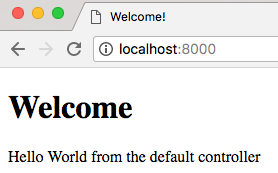
\includegraphics{./tex2pdf.-05a85d9d563be472/a97f353efafa2faa98064075e63812a2b1cec288.png}
\caption{Home page. \label{homepage}}
\end{figure}

\hypertarget{using-the-make-tool-to-create-a-web-test}{%
\section{Using the `make' tool to create a web
test}\label{using-the-make-tool-to-create-a-web-test}}

The Symfony console `make' tool can be used to create web test classes:

\begin{Shaded}
\begin{Highlighting}[]
\NormalTok{    $ }\ExtensionTok{symfony}\NormalTok{ console make:test}

    \ExtensionTok{//}\NormalTok{ choose }\StringTok{'WebTestCase'}\NormalTok{ when asked:}

     \ExtensionTok{Which}\NormalTok{ test type would you like?:}
\NormalTok{      [}\ExtensionTok{TestCase}\NormalTok{       ] basic PHPUnit tests}
\NormalTok{      [}\ExtensionTok{KernelTestCase}\NormalTok{ ] basic tests that have access to Symfony services}
\NormalTok{      [}\ExtensionTok{WebTestCase}\NormalTok{    ] to run browser-like scenarios, but that don}\StringTok{'t execute JavaScript code}
\StringTok{      [ApiTestCase    ] to run API-oriented scenarios}
\StringTok{      [PantherTestCase] to run e2e scenarios, using a real-browser or HTTP client and a real web server}
\StringTok{     > WebTestCase}

\StringTok{    // name the new class '}\NormalTok{HomePageTest}\StringTok{' when asked:}

\StringTok{    Choose a class name for your test, like:}
\StringTok{     * UtilTest (to create tests/UtilTest.php)}
\StringTok{     * Service\textbackslash{}UtilTest (to create tests/Service/UtilTest.php)}
\StringTok{     * \textbackslash{}App\textbackslash{}Tests\textbackslash{}Service\textbackslash{}UtilTest (to create tests/Service/UtilTest.php)}

\StringTok{     The name of the test class (e.g. BlogPostTest):}
\StringTok{     > HomePageTest}

\StringTok{     created: tests/HomePageTest.php}

\StringTok{      Success!}

\StringTok{     Next: Open your new test class and start customizing it.}
\StringTok{     Find the documentation at https://symfony.com/doc/current/testing.html#functional-tests}

\end{Highlighting}
\end{Shaded}

\hypertarget{automating-a-test-for-the-home-page-contents}{%
\section{Automating a test for the home page
contents}\label{automating-a-test-for-the-home-page-contents}}

Let's write a test class for our \texttt{DefaultController} class. So we
create a new test class
\texttt{/tests/Controller/DefaultControllerTest.php}. We'll write 2
tests, one to check that we get a 200 OK HTTP success code when we try
to request \texttt{/}, and secondly that the content received in the
HTTP Response contains the text \texttt{Hello\ World}:

\begin{Shaded}
\begin{Highlighting}[]
    \KeywordTok{namespace}\NormalTok{ App\textbackslash{}Tests\textbackslash{}Controller}\OtherTok{;}

    \KeywordTok{use}\NormalTok{ Symfony\textbackslash{}Bundle\textbackslash{}FrameworkBundle\textbackslash{}Test\textbackslash{}WebTestCase}\OtherTok{;}
    \KeywordTok{use}\NormalTok{ Symfony\textbackslash{}Component\textbackslash{}HttpFoundation\textbackslash{}Response}\OtherTok{;}

    \KeywordTok{class}\NormalTok{ DefaultControllerTest }\KeywordTok{extends}\NormalTok{ WebTestCase}
\NormalTok{    \{}
        \CommentTok{// methods go here}
\NormalTok{    \}}
\end{Highlighting}
\end{Shaded}

We see our class must extend \texttt{WebTestCase} from package
\texttt{Symfony\textbackslash{}Bundle\textbackslash{}FrameworkBundle\textbackslash{}Test\textbackslash{}},
and also makes use of the Symfony Foundation \texttt{Response} class.

Our method to test for a 200 OK Response code is as follows:

\begin{Shaded}
\begin{Highlighting}[]

    \KeywordTok{public} \KeywordTok{function}\NormalTok{ testHomepageResponseCodeOkay}\OtherTok{()}
\NormalTok{    \{}
        \CommentTok{// Arrange}
        \KeywordTok{$url}\NormalTok{ = }\StringTok{'/'}\OtherTok{;}
        \KeywordTok{$httpMethod}\NormalTok{ = }\StringTok{'GET'}\OtherTok{;}
        \KeywordTok{$client}\NormalTok{ = }\KeywordTok{static}\NormalTok{::createClient}\OtherTok{();}

        \CommentTok{// Assert}
        \KeywordTok{$client}\NormalTok{->request}\OtherTok{(}\KeywordTok{$httpMethod}\OtherTok{,} \KeywordTok{$url}\OtherTok{);}
        \KeywordTok{$statusCode}\NormalTok{ = }\KeywordTok{$client}\NormalTok{->getResponse}\OtherTok{()}\NormalTok{->getStatusCode}\OtherTok{();}

        \CommentTok{// Assert}
        \KeywordTok{$this}\NormalTok{->assertSame}\OtherTok{(}\NormalTok{Response::}\KeywordTok{HTTP_OK}\OtherTok{,} \KeywordTok{$statusCode}\OtherTok{);}
\NormalTok{    \}}
\end{Highlighting}
\end{Shaded}

NOTE: Another way to check the Response status code is to use the
\texttt{\$this-\textgreater{}assertResponseStatusCodeSame(\textless{}code\textgreater{})}
method. For example:

\begin{Shaded}
\begin{Highlighting}[]
    \KeywordTok{$this}\NormalTok{->assertResponseStatusCodeSame}\OtherTok{(}\NormalTok{Response::}\KeywordTok{HTTP_OK}\OtherTok{);}
\end{Highlighting}
\end{Shaded}

We see how a web client object \texttt{\$client} is created and makes a
GET request to \texttt{/}. We see how we can interrogate the contents of
the HTTP Response received using the \texttt{getResponse()} method, and
within that we can extract the status code, and compare with the class
constant \texttt{HTTP\_OK} (200).

Here is our method to test for a Level 1 heading containing
\textbf{exactly} \texttt{Hello\ World} (case sensitive):

\begin{Shaded}
\begin{Highlighting}[]
    \KeywordTok{public} \KeywordTok{function}\NormalTok{ testHomepageContentContainsHelloWorld}\OtherTok{()}\NormalTok{: }\KeywordTok{void}
\NormalTok{    \{}
        \CommentTok{// Arrange}
        \KeywordTok{$url}\NormalTok{ = }\StringTok{'/'}\OtherTok{;}
        \KeywordTok{$httpMethod}\NormalTok{ = }\StringTok{'GET'}\OtherTok{;}
        \KeywordTok{$client}\NormalTok{ = }\KeywordTok{static}\NormalTok{::createClient}\OtherTok{();}
        \KeywordTok{$searchText}\NormalTok{ = }\StringTok{'Hello World'}\OtherTok{;}
        \KeywordTok{$cssSelector}\NormalTok{ = }\StringTok{'h1'}\OtherTok{;}

        \CommentTok{// Act}
        \KeywordTok{$crawler}\NormalTok{ = }\KeywordTok{$client}\NormalTok{->request}\OtherTok{(}\KeywordTok{$httpMethod}\OtherTok{,} \KeywordTok{$url}\OtherTok{);}
        \KeywordTok{$content}\NormalTok{ = }\KeywordTok{$client}\NormalTok{->getResponse}\OtherTok{()}\NormalTok{->getContent}\OtherTok{();}

        \CommentTok{// Assert}
        \KeywordTok{$this}\NormalTok{->assertResponseIsSuccessful}\OtherTok{();}
        \KeywordTok{$this}\NormalTok{->assertSelectorTextContains}\OtherTok{(}\KeywordTok{$cssSelector}\OtherTok{,} \KeywordTok{$searchText}\OtherTok{);}
\NormalTok{    \}}
\end{Highlighting}
\end{Shaded}

We see how we can use the \texttt{assertSelectorTextContains} string
method to search for the string \texttt{Hello\ World} in the content of
the HTTP Response.

When we run PHPUnit we can see success both from the full-stops at the
CLI, and in our log files. For example we case see the human-friendly
\texttt{teestdox} report in \texttt{/build/testdox.txt} as follows:

\begin{verbatim}
    Default Controller (App\Tests\Controller\DefaultController)
     [x] Homepage response code okay
     [x] Homepage content contains hello world
\end{verbatim}

\hypertarget{testing-text-case-insensitively}{%
\section{Testing text
case-insensitively}\label{testing-text-case-insensitively}}

I lost 30 minutes thinking my web app wasn't working! This was due to
the difference between \texttt{Hello\ world} and \texttt{Hello\ World}:
{[}w{]}orld vs {[}W{]}orld.

Luckily there is a specific assertion for testing text that ignores
case:

\begin{itemize}
\tightlist
\item
  \texttt{assertStringContainsStringIgnoringCase(\textless{}needle\textgreater{},\ \textless{}haystack\textgreater{})}
\end{itemize}

Here's a full test method for case insensitively:

\begin{Shaded}
\begin{Highlighting}[]
    \KeywordTok{public} \KeywordTok{function}\NormalTok{ testHomepageContentContainsHelloWorldIgnoreCase}\OtherTok{()}
\NormalTok{    \{}
        \CommentTok{// Arrange}
        \KeywordTok{$url}\NormalTok{ = }\StringTok{'/'}\OtherTok{;}
        \KeywordTok{$httpMethod}\NormalTok{ = }\StringTok{'GET'}\OtherTok{;}
        \KeywordTok{$client}\NormalTok{ = }\KeywordTok{static}\NormalTok{::createClient}\OtherTok{();}
        \KeywordTok{$searchText}\NormalTok{ = }\StringTok{'heLLo worLD'}\OtherTok{;}
        \KeywordTok{$cssSelector}\NormalTok{ = }\StringTok{'body'}\OtherTok{;}

        \CommentTok{// Act}
        \KeywordTok{$crawler}\NormalTok{ = }\KeywordTok{$client}\NormalTok{->request}\OtherTok{(}\KeywordTok{$httpMethod}\OtherTok{,} \KeywordTok{$url}\OtherTok{);}
        \KeywordTok{$content}\NormalTok{ = }\KeywordTok{$client}\NormalTok{->getResponse}\OtherTok{()}\NormalTok{->getContent}\OtherTok{();}

        \CommentTok{// Assert}
        \KeywordTok{$this}\NormalTok{->assertStringContainsStringIgnoringCase}\OtherTok{(}\KeywordTok{$searchText}\OtherTok{,} \KeywordTok{$content}\OtherTok{);}
\NormalTok{    \}}
\end{Highlighting}
\end{Shaded}

\hypertarget{test-multiple-pages-with-a-data-provider}{%
\section{Test multiple pages with a data
provider}\label{test-multiple-pages-with-a-data-provider}}

Avoid duplicating code when only the URL and search text changes, by
writing a testing method fed by arrays of test input / expected values
from a data provider method.

Here is a method with a provider, testing for \texttt{hello\ world} in
the home page (route \texttt{/}), and \texttt{about} for the
\texttt{/about} route:

\begin{Shaded}
\begin{Highlighting}[]
    \CommentTok{/**}
\CommentTok{     * }\AnnotationTok{@dataProvider}\CommentTok{ basicPagesTextProvider}
\CommentTok{     */}
    \KeywordTok{public} \KeywordTok{function}\NormalTok{ testPublicPagesContainBasicText}\OtherTok{(}\KeywordTok{string} \KeywordTok{$url}\OtherTok{,} \KeywordTok{string} \KeywordTok{$searchText}\OtherTok{)}
\NormalTok{    \{}
        \CommentTok{// Arrange}
        \KeywordTok{$httpMethod}\NormalTok{ = }\StringTok{'GET'}\OtherTok{;}
        \KeywordTok{$client}\NormalTok{ = }\KeywordTok{static}\NormalTok{::createClient}\OtherTok{();}

        \CommentTok{// Act}
        \KeywordTok{$crawler}\NormalTok{ = }\KeywordTok{$client}\NormalTok{->request}\OtherTok{(}\KeywordTok{$httpMethod}\OtherTok{,} \KeywordTok{$url}\OtherTok{);}
        \KeywordTok{$content}\NormalTok{ = }\KeywordTok{$client}\NormalTok{->getResponse}\OtherTok{()}\NormalTok{->getContent}\OtherTok{();}

        \CommentTok{// Assert}
        \KeywordTok{$this}\NormalTok{->assertStringContainsStringIgnoringCase}\OtherTok{(}\KeywordTok{$searchText}\OtherTok{,} \KeywordTok{$content}\OtherTok{);}
\NormalTok{    \}}

    \KeywordTok{public} \KeywordTok{function}\NormalTok{ basicPagesTextProvider}\OtherTok{()}\NormalTok{: }\KeywordTok{array}
\NormalTok{    \{}
        \KeywordTok{return} \OtherTok{[}
            \OtherTok{[}\StringTok{'/'}\OtherTok{,} \StringTok{'hello WORLD'}\OtherTok{],}
            \OtherTok{[}\StringTok{'/about'}\OtherTok{,} \StringTok{'about'}\OtherTok{],}
        \OtherTok{];}
\NormalTok{    \}}
\end{Highlighting}
\end{Shaded}

\hypertarget{count-the-number-of-elements}{%
\section{Count the number of
elements}\label{count-the-number-of-elements}}

We can use the \texttt{filter(...)} method of the crawler object to
retrieve an array of elements matching a CSS selector.

For example, this statement asserts that there should be exactly 4
elements with CSS class \texttt{comment}:

\begin{Shaded}
\begin{Highlighting}[]
    \KeywordTok{$this}\NormalTok{->assertCount}\OtherTok{(}\DecValTok{4}\OtherTok{,} \KeywordTok{$crawler}\NormalTok{->filter}\OtherTok{(}\StringTok{'.comment'}\OtherTok{));}
\end{Highlighting}
\end{Shaded}

\hypertarget{testing-different-content-returned-by-the-response}{%
\section{Testing different content returned by the
Response}\label{testing-different-content-returned-by-the-response}}

Our test classes are subclasses of the Symfony \texttt{WebTestCase}
class, which provides a number of methods for testing the contents of
the HTTP Response.

So there are several useful assertions we can make based on CSS element
selectors, including:

\begin{itemize}
\item
  \texttt{\$this-\textgreater{}assertSelectorExists(\$cssSelector)}

  \begin{itemize}
  \tightlist
  \item
    this assets that a given element is present in the Response content
    (such as \texttt{\#formHeading}, \texttt{h1}, \texttt{title},
    \texttt{body} etc.)
  \end{itemize}
\item
  \texttt{\$this-\textgreater{}assertSelectorNOTExists(\$cssSelector)}

  \begin{itemize}
  \tightlist
  \item
    as above but that the selector is NOT present in the Response
  \end{itemize}
\item
  \texttt{\$this-\textgreater{}assertSelectorTextContains(\$cssSelector,\ \$searchText)}

  \begin{itemize}
  \tightlist
  \item
    this assets that a given element (such as \texttt{h1},
    \texttt{title}, \texttt{body} etc.) contains some given text
  \end{itemize}
\item
  \texttt{\$this-\textgreater{}assertSelectorTextNotContains(\$cssSelector,\ \$searchText)}

  \begin{itemize}
  \tightlist
  \item
    as above but that the search text is NOT present in selected element
    of the Response
  \end{itemize}
\item
  \texttt{\$this-\textgreater{}assertSelectorTextSame(\$cssSelector,\ \$searchText)}

  \begin{itemize}
  \tightlist
  \item
    this assets that a given element (such as \texttt{h1},
    \texttt{title}, \texttt{body} etc.) contains some given text
  \end{itemize}
\end{itemize}

Here we see a test with many of these assertions demonstrated:

\begin{Shaded}
\begin{Highlighting}[]
    \KeywordTok{public} \KeywordTok{function}\NormalTok{ testHomepageBodyContentContainsHelloAndNotDinasaur}\OtherTok{()}\NormalTok{: }\KeywordTok{void}
\NormalTok{    \{}
        \CommentTok{// Arrange}
        \KeywordTok{$url}\NormalTok{ = }\StringTok{'/'}\OtherTok{;}
        \KeywordTok{$httpMethod}\NormalTok{ = }\StringTok{'GET'}\OtherTok{;}
        \KeywordTok{$client}\NormalTok{ = }\KeywordTok{static}\NormalTok{::createClient}\OtherTok{();}
        \KeywordTok{$searchText}\NormalTok{ = }\StringTok{'Hello World'}\OtherTok{;}
        \KeywordTok{$textNotInPage}\NormalTok{ = }\StringTok{'Dinosaur'}\OtherTok{;}
        \KeywordTok{$cssSelector}\NormalTok{ = }\StringTok{'body'}\OtherTok{;}

        \CommentTok{// Act}
        \KeywordTok{$crawler}\NormalTok{ = }\KeywordTok{$client}\NormalTok{->request}\OtherTok{(}\KeywordTok{$httpMethod}\OtherTok{,} \KeywordTok{$url}\OtherTok{);}
        \KeywordTok{$content}\NormalTok{ = }\KeywordTok{$client}\NormalTok{->getResponse}\OtherTok{()}\NormalTok{->getContent}\OtherTok{();}

        \CommentTok{// Assert}
        \KeywordTok{$this}\NormalTok{->assertResponseIsSuccessful}\OtherTok{();}

        \CommentTok{// has a 'body' element}
        \KeywordTok{$this}\NormalTok{->assertSelectorExists}\OtherTok{(}\KeywordTok{$cssSelector}\OtherTok{);}

        \CommentTok{// does NOT have a 'footer' element}
        \KeywordTok{$this}\NormalTok{->assertSelectorNotExists}\OtherTok{(}\StringTok{'footer'}\OtherTok{);}

        \CommentTok{// 'body' contains 'Hello'}
        \KeywordTok{$this}\NormalTok{->assertSelectorTextContains}\OtherTok{(}\KeywordTok{$cssSelector}\OtherTok{,} \KeywordTok{$searchText}\OtherTok{);}

        \CommentTok{// 'body' dopes NOT contains 'Dinosaur'}
        \KeywordTok{$this}\NormalTok{->assertSelectorTextNotContains}\OtherTok{(}\KeywordTok{$cssSelector}\OtherTok{,} \KeywordTok{$textNotInPage}\OtherTok{);}

        \CommentTok{// 'h1' exact text of 'Hello World'}
        \KeywordTok{$this}\NormalTok{->assertSelectorTextSame}\OtherTok{(}\StringTok{'h1'}\OtherTok{,} \KeywordTok{$searchText}\OtherTok{);}
\NormalTok{    \}}
\end{Highlighting}
\end{Shaded}

\hypertarget{testing-route-followed-after-link-clicked-or-form-submission}{%
\section{Testing route followed after link clicked or form
submission}\label{testing-route-followed-after-link-clicked-or-form-submission}}

Another useful assertion is
\texttt{\$this-\textgreater{}assertRouteSame(\textless{}routeName\textgreater{})}
which asserts that the Response now received is from a link or redirect
followed, corresponding to the given route name.

For example, the following test checks that after clicking the
\texttt{/about} link, the Response is from the \texttt{/about} route
(more about links in the next section):

\begin{Shaded}
\begin{Highlighting}[]
    \KeywordTok{public} \KeywordTok{function}\NormalTok{ testHomepageResponseProperties}\OtherTok{()}\NormalTok{: }\KeywordTok{void}
\NormalTok{    \{}
        \CommentTok{// Arrange}
        \KeywordTok{$url}\NormalTok{ = }\StringTok{'/'}\OtherTok{;}
        \KeywordTok{$httpMethod}\NormalTok{ = }\StringTok{'GET'}\OtherTok{;}
        \KeywordTok{$client}\NormalTok{ = }\KeywordTok{static}\NormalTok{::createClient}\OtherTok{();}
        \KeywordTok{$client}\NormalTok{->followRedirects}\OtherTok{();}
        \KeywordTok{$homeRoute}\NormalTok{ = }\StringTok{'home'}\OtherTok{;}
        \KeywordTok{$aboutRoute}\NormalTok{ = }\StringTok{'about'}\OtherTok{;}

        \CommentTok{// Act}
        \KeywordTok{$crawler}\NormalTok{ = }\KeywordTok{$client}\NormalTok{->request}\OtherTok{(}\KeywordTok{$httpMethod}\OtherTok{,} \KeywordTok{$url}\OtherTok{);}

        \CommentTok{// click ABOUT link}
        \KeywordTok{$linkText}\NormalTok{ = }\StringTok{'about'}\OtherTok{;}
        \KeywordTok{$link}\NormalTok{ = }\KeywordTok{$crawler}\NormalTok{->selectLink}\OtherTok{(}\KeywordTok{$linkText}\OtherTok{)}\NormalTok{->}\FunctionTok{link}\OtherTok{();}
        \KeywordTok{$client}\NormalTok{->click}\OtherTok{(}\KeywordTok{$link}\OtherTok{);}

        \CommentTok{// now on page for about route}
        \KeywordTok{$this}\NormalTok{->assertRouteSame}\OtherTok{(}\KeywordTok{$aboutRoute}\OtherTok{);}
\NormalTok{    \}}
\end{Highlighting}
\end{Shaded}

\hypertarget{testing-links-project-test05}{%
\section{\texorpdfstring{Testing links (project
\texttt{test05})}{Testing links (project test05)}}\label{testing-links-project-test05}}

We can test links with our web crawler as follows:

\begin{itemize}
\item
  get reference to crawler object when you make the initial request

\begin{verbatim}
$httpMethod = 'GET';
$url = '/about';
$crawler = $client->request($httpMethod, $url);
\end{verbatim}
\item
  select a link with:

\begin{verbatim}
$linkText = 'login';
$link = $crawler->selectLink($linkText)->link();
\end{verbatim}
\item
  click the link with:

\begin{verbatim}
$client->click($link);
\end{verbatim}
\item
  then check the content of the new request

\begin{verbatim}

// set $expectedText to what should in page when link has been followed ...
// Assert
$content = $client->getResponse()->getContent();
$this->assertStringContainsString($expectedText, $content);

$this->assertSelectorTextContains($cssSelector, $expectedText);
\end{verbatim}
\end{itemize}

For example, if we create a new `about' page Twig template
`/templates/default/about.html.twig':

\begin{verbatim}
    

    
    <h1>About page</h1>

        <p>
            About this great website!
        </p>

    
\end{verbatim}

and a \texttt{DefaultController} method to display this page when the
route matches \texttt{/about}:

\begin{Shaded}
\begin{Highlighting}[]
    \CommentTok{#[Route('/about', name: 'about')]}
    \KeywordTok{public} \KeywordTok{function}\NormalTok{ about}\OtherTok{()}\NormalTok{: Response}
\NormalTok{    \{}
        \KeywordTok{$template}\NormalTok{ = }\StringTok{'default/about.html.twig'}\OtherTok{;}
        \KeywordTok{$args}\NormalTok{ = }\OtherTok{[];}
        \KeywordTok{return} \KeywordTok{$this}\NormalTok{->render}\OtherTok{(}\KeywordTok{$template}\OtherTok{,} \KeywordTok{$args}\OtherTok{);}
\NormalTok{    \}}
\end{Highlighting}
\end{Shaded}

If we add to our base Twig template links to the homepage and the about,
in template \texttt{/templates/base.html.twig}:

\begin{verbatim}
    <!DOCTYPE html>
    <html>
        <head>
            <meta charset="UTF-8">
            <title>Welcome!</title>
            
        </head>
        <body>

        <nav>
            <ul>
                <li>
                    <a href="{{ url('homepage') }}">home</a>
                </li>
                <li>
                    <a href="{{ url('about') }}">about</a>
                </li>
            </ul>
        </nav>

            
        </body>
    </html>
\end{verbatim}

We can now write a test method to:

\begin{itemize}
\item
  request the homepage \texttt{/}
\item
  select and click the \texttt{about} link
\item
  test that the content of the new response is the `about' page if it
  contains `about page'
\end{itemize}

Here is our test method:

\begin{Shaded}
\begin{Highlighting}[]
    \KeywordTok{public} \KeywordTok{function}\NormalTok{ testHomePageLinkToAboutWorks}\OtherTok{()}
\NormalTok{    \{}
        \CommentTok{// Arrange}
        \KeywordTok{$url}\NormalTok{ = }\StringTok{'/'}\OtherTok{;}
        \KeywordTok{$httpMethod}\NormalTok{ = }\StringTok{'GET'}\OtherTok{;}
        \KeywordTok{$client}\NormalTok{ = }\KeywordTok{static}\NormalTok{::createClient}\OtherTok{();}
        \KeywordTok{$client}\NormalTok{->followRedirects}\OtherTok{();}
        \KeywordTok{$searchText}\NormalTok{ = }\StringTok{'About'}\OtherTok{;}
        \KeywordTok{$linkText}\NormalTok{ = }\StringTok{'about'}\OtherTok{;}
        \KeywordTok{$cssSelector}\NormalTok{ = }\StringTok{'body'}\OtherTok{;}

        \CommentTok{// Act}
        \KeywordTok{$crawler}\NormalTok{ = }\KeywordTok{$client}\NormalTok{->request}\OtherTok{(}\KeywordTok{$httpMethod}\OtherTok{,} \KeywordTok{$url}\OtherTok{);}
        \KeywordTok{$link}\NormalTok{ = }\KeywordTok{$crawler}\NormalTok{->selectLink}\OtherTok{(}\KeywordTok{$linkText}\OtherTok{)}\NormalTok{->}\FunctionTok{link}\OtherTok{();}
        \KeywordTok{$client}\NormalTok{->click}\OtherTok{(}\KeywordTok{$link}\OtherTok{);}
        \KeywordTok{$content}\NormalTok{ = }\KeywordTok{$client}\NormalTok{->getResponse}\OtherTok{()}\NormalTok{->getContent}\OtherTok{();}

        \CommentTok{// Assert}
        \KeywordTok{$this}\NormalTok{->assertStringContainsString}\OtherTok{(}\KeywordTok{$searchText}\OtherTok{,} \KeywordTok{$content}\OtherTok{);}

        \KeywordTok{$this}\NormalTok{->assertSelectorTextContains}\OtherTok{(}\KeywordTok{$cssSelector}\OtherTok{,} \KeywordTok{$searchText}\OtherTok{);}
\NormalTok{    \}}
\end{Highlighting}
\end{Shaded}

\hypertarget{instruct-client-to-follow-redirects}{%
\subsection{Instruct client to `follow
redirects'}\label{instruct-client-to-follow-redirects}}

In most cases we want our testing web-crawler client to follow
redirects. So we need to add the
\texttt{\$client-\textgreater{}followRedirects(true)} statement
immediately after creating the client object.

\begin{Shaded}
\begin{Highlighting}[]
    \KeywordTok{public} \KeywordTok{function}\NormalTok{ testExchangePage}\OtherTok{()}
\NormalTok{    \{}
        \KeywordTok{$httpMethod}\NormalTok{ = }\StringTok{'GET'}\OtherTok{;}
        \KeywordTok{$url}\NormalTok{ = }\StringTok{'/calc'}\OtherTok{;}
        \KeywordTok{$client}\NormalTok{ = }\KeywordTok{static}\NormalTok{::createClient}\OtherTok{();}
        \KeywordTok{$client}\NormalTok{->followRedirects}\OtherTok{();} \CommentTok{// <<<<<<<<<<<<<<<< default is 'true'}
        \KeywordTok{$client}\NormalTok{->request}\OtherTok{(}\KeywordTok{$httpMethod}\OtherTok{,} \KeywordTok{$url}\OtherTok{);}
        \KeywordTok{$this}\NormalTok{->assertSame}\OtherTok{(}\NormalTok{Response::}\KeywordTok{HTTP_OK}\OtherTok{,} \KeywordTok{$client}\NormalTok{->getResponse}\OtherTok{()}\NormalTok{->getStatusCode}\OtherTok{());}
\NormalTok{    \}}
\end{Highlighting}
\end{Shaded}

\hypertarget{testing-web-forms}{%
\chapter{Testing web forms}\label{testing-web-forms}}

\hypertarget{testing-forms-project-test06}{%
\section{\texorpdfstring{Testing forms (project
\texttt{test06})}{Testing forms (project test06)}}\label{testing-forms-project-test06}}

Testing forms is similar to testing links, in that we need to get a
reference to the form (via its submit button), then insert out data,
then submit the form, and examine the content of the new response
received after the form submission.

Assume we have a Calculator class as follows in
\texttt{/src/Util/Calculator.php}:

\begin{Shaded}
\begin{Highlighting}[]
    \KeywordTok{namespace}\NormalTok{ App\textbackslash{}Util}\OtherTok{;}

    \KeywordTok{class}\NormalTok{ Calculator}
\NormalTok{    \{}
        \KeywordTok{public} \KeywordTok{function}\NormalTok{ add}\OtherTok{(}\KeywordTok{$n1}\OtherTok{,} \KeywordTok{$n2}\OtherTok{)}
\NormalTok{        \{}
            \KeywordTok{return} \KeywordTok{$n1}\NormalTok{ + }\KeywordTok{$n2}\OtherTok{;}
\NormalTok{        \}}

        \KeywordTok{public} \KeywordTok{function}\NormalTok{ subtract}\OtherTok{(}\KeywordTok{$n1}\OtherTok{,} \KeywordTok{$n2}\OtherTok{)}
\NormalTok{        \{}
            \KeywordTok{return} \KeywordTok{$n1}\NormalTok{ - }\KeywordTok{$n2}\OtherTok{;}
\NormalTok{        \}}

        \KeywordTok{public} \KeywordTok{function}\NormalTok{ divide}\OtherTok{(}\KeywordTok{$n}\OtherTok{,} \KeywordTok{$divisor}\OtherTok{)}
\NormalTok{        \{}
            \KeywordTok{if}\OtherTok{(}\KeywordTok{empty}\OtherTok{(}\KeywordTok{$divisor}\OtherTok{))}\NormalTok{\{}
                \KeywordTok{throw} \KeywordTok{new}\NormalTok{ \textbackslash{}}\KeywordTok{InvalidArgumentException}\OtherTok{(}\StringTok{"Divisor must be a number"}\OtherTok{);}
\NormalTok{            \}}

            \KeywordTok{return} \KeywordTok{$n}\NormalTok{ / }\KeywordTok{$divisor}\OtherTok{;}
\NormalTok{        \}}

        \KeywordTok{public} \KeywordTok{function}\NormalTok{ process}\OtherTok{(}\KeywordTok{$n1}\OtherTok{,} \KeywordTok{$n2}\OtherTok{,} \KeywordTok{$process}\OtherTok{)}
\NormalTok{        \{}
            \KeywordTok{switch}\OtherTok{(}\KeywordTok{$process}\OtherTok{)}\NormalTok{\{}
                \KeywordTok{case }\StringTok{'subtract'}\OtherTok{:}
                    \KeywordTok{return} \KeywordTok{$this}\NormalTok{->subtract}\OtherTok{(}\KeywordTok{$n1}\OtherTok{,} \KeywordTok{$n2}\OtherTok{);}
                    \KeywordTok{break}\OtherTok{;}
                \KeywordTok{case }\StringTok{'divide'}\OtherTok{:}
                    \KeywordTok{return} \KeywordTok{$this}\NormalTok{->divide}\OtherTok{(}\KeywordTok{$n1}\OtherTok{,} \KeywordTok{$n2}\OtherTok{);}
                    \KeywordTok{break}\OtherTok{;}
                \KeywordTok{case }\StringTok{'add'}\OtherTok{:}
                \KeywordTok{default:}
                    \KeywordTok{return} \KeywordTok{$this}\NormalTok{->add}\OtherTok{(}\KeywordTok{$n1}\OtherTok{,} \KeywordTok{$n2}\OtherTok{);}
\NormalTok{            \}}
\NormalTok{        \}}
\NormalTok{    \}}
\end{Highlighting}
\end{Shaded}

Assume we also have a \texttt{CalculatorController} class in
\texttt{/src/Controller/}:

\begin{Shaded}
\begin{Highlighting}[]
    \KeywordTok{namespace}\NormalTok{ App\textbackslash{}Controller}\OtherTok{;}

    \KeywordTok{use}\NormalTok{ App\textbackslash{}Util\textbackslash{}Calculator}\OtherTok{;}
    \KeywordTok{use}\NormalTok{ Symfony\textbackslash{}Component\textbackslash{}Routing\textbackslash{}Annotation\textbackslash{}Route}\OtherTok{;}
    \KeywordTok{use}\NormalTok{ Symfony\textbackslash{}Bundle\textbackslash{}FrameworkBundle\textbackslash{}Controller\textbackslash{}Controller}\OtherTok{;}
    \KeywordTok{use}\NormalTok{ Symfony\textbackslash{}Component\textbackslash{}HttpFoundation\textbackslash{}Request}\OtherTok{;}

    \KeywordTok{class}\NormalTok{ CalcController }\KeywordTok{extends}\NormalTok{ Controller}
\NormalTok{    \{}
        \StringTok{...}\NormalTok{ methods go here }\StringTok{...}
\NormalTok{    \}}
\end{Highlighting}
\end{Shaded}

There is a calculator home page that displays the form Twig template at
\texttt{/templates/calc/index.html.twig}:

\begin{Shaded}
\begin{Highlighting}[]
    \CommentTok{#[Route('/calculator', name: 'app_calculator_index')]}
    \KeywordTok{public} \KeywordTok{function}\NormalTok{ index}\OtherTok{()}\NormalTok{: Response}
\NormalTok{    \{}
        \KeywordTok{$template}\NormalTok{ = }\StringTok{'calculator/index.html.twig'}\OtherTok{;}
        \KeywordTok{$args}\NormalTok{ = }\OtherTok{[];}
        \KeywordTok{return} \KeywordTok{$this}\NormalTok{->render}\OtherTok{(}\KeywordTok{$template}\OtherTok{,} \KeywordTok{$args}\OtherTok{);}
\NormalTok{    \}}
\end{Highlighting}
\end{Shaded}

and a `process' controller method to received the form data (n1, n2,
operator) and process it: There is a calculator home page that displays
the form Twig template at
\texttt{/templates/calculator/index.html.twig}:

\begin{Shaded}
\begin{Highlighting}[]

    \KeywordTok{use}\NormalTok{ Symfony\textbackslash{}Component\textbackslash{}HttpFoundation\textbackslash{}Request}\OtherTok{;}
    \KeywordTok{use}\NormalTok{ App\textbackslash{}Util\textbackslash{}Calculator}\OtherTok{;}

    \StringTok{...}

    \CommentTok{#[Route('/calculator/process', name: 'app_calculator_process')]}
    \KeywordTok{public} \KeywordTok{function}\NormalTok{ processAction}\OtherTok{(}\NormalTok{Request }\KeywordTok{$request}\OtherTok{)}\NormalTok{: Response}
\NormalTok{    \{}
        \CommentTok{// extract name values from POST data}
        \KeywordTok{$n1}\NormalTok{ = }\KeywordTok{$request}\NormalTok{->request->get}\OtherTok{(}\StringTok{'num1'}\OtherTok{);}
        \KeywordTok{$n2}\NormalTok{ = }\KeywordTok{$request}\NormalTok{->request->get}\OtherTok{(}\StringTok{'num2'}\OtherTok{);}
        \KeywordTok{$operator}\NormalTok{ = }\KeywordTok{$request}\NormalTok{->request->get}\OtherTok{(}\StringTok{'operator'}\OtherTok{);}

        \KeywordTok{$calc}\NormalTok{ = }\KeywordTok{new}\NormalTok{ Calculator}\OtherTok{();}
        \KeywordTok{$answer}\NormalTok{ = }\KeywordTok{$calc}\NormalTok{->process}\OtherTok{(}\KeywordTok{$n1}\OtherTok{,} \KeywordTok{$n2}\OtherTok{,} \KeywordTok{$operator}\OtherTok{);}

        \KeywordTok{$template}\NormalTok{ = }\StringTok{'calculator/result.html.twig'}\OtherTok{;}
        \KeywordTok{$args}\NormalTok{ =  }\OtherTok{[}
            \StringTok{'n1'}\NormalTok{ => }\KeywordTok{$n1}\OtherTok{,}
            \StringTok{'n2'}\NormalTok{ => }\KeywordTok{$n2}\OtherTok{,}
            \StringTok{'operator'}\NormalTok{ => }\KeywordTok{$operator}\OtherTok{,}
            \StringTok{'answer'}\NormalTok{ => }\KeywordTok{$answer}
        \OtherTok{];}

        \KeywordTok{return} \KeywordTok{$this}\NormalTok{->render}\OtherTok{(}\KeywordTok{$template}\OtherTok{,} \KeywordTok{$args}\OtherTok{);}
\NormalTok{    \}}
\end{Highlighting}
\end{Shaded}

The Twig template to display our form looks as follows
\texttt{/templates/calculator/index.html.twig}:

\begin{verbatim}
    

    
    <h1>Calculator home</h1>

        <form method="post" action="{{ url('app_calculator_process') }}">
            <p>
                Num 1:
                <input type="text" name="num1" value="1">
            </p>
            <p>
                Num 2:
                <input type="text" name="num2" value="1">
            </p>
            <p>
                Operation:
                <br>
                ADD
                <input type="radio" name="operator" value="add" checked>
                <br>
                SUBTRACT
                <input type="radio" name="operator" value="subtract">
                <br>
                DIVIDE
                <input type="radio" name="operator" value="divide">
            </p>

            <p>
                <input type="submit" name="calc_submit">
            </p>
        </form>

    
\end{verbatim}

and the Twig template to confirm received values, and display the answer
\texttt{result.html.twig} contains:

\begin{verbatim}
    <h1>Calc RESULT</h1>
    <p>
        Your inputs were:
        <br>
        n1 = {{ n1 }}
        <br>
        n2 = {{ n2 }}
        <br>
        operator = {{ operator }}
    <p>
        answer = {{ answer }}
\end{verbatim}

\hypertarget{create-a-calculatortest-class}{%
\section{\texorpdfstring{Create a \texttt{CalculatorTest}
class}{Create a CalculatorTest class}}\label{create-a-calculatortest-class}}

Using the Symfony make tool, let's create a \texttt{CalculatorTest}
class in \texttt{/src/Tests/}:

\begin{Shaded}
\begin{Highlighting}[]
    \VariableTok{$symfony} \ExtensionTok{console}\NormalTok{ make:test}

     \ExtensionTok{Which}\NormalTok{ test type would you like?:}
\NormalTok{      [}\ExtensionTok{TestCase}\NormalTok{       ] basic PHPUnit tests}
\NormalTok{      [}\ExtensionTok{KernelTestCase}\NormalTok{ ] basic tests that have access to Symfony services}
\NormalTok{      [}\ExtensionTok{WebTestCase}\NormalTok{    ] to run browser-like scenarios, but that don}\StringTok{'t execute JavaScript code}
\StringTok{      [ApiTestCase    ] to run API-oriented scenarios}
\StringTok{      [PantherTestCase] to run e2e scenarios, using a real-browser or HTTP client and a real web server}
\StringTok{     > WebTestCase}


\StringTok{    Choose a class name for your test, like:}
\StringTok{     * UtilTest (to create tests/UtilTest.php)}
\StringTok{     * Service\textbackslash{}UtilTest (to create tests/Service/UtilTest.php)}
\StringTok{     * \textbackslash{}App\textbackslash{}Tests\textbackslash{}Service\textbackslash{}UtilTest (to create tests/Service/UtilTest.php)}

\StringTok{     The name of the test class (e.g. BlogPostTest):}
\StringTok{     > CalculatorTest}

\StringTok{     created: tests/CalculatorTest.php}

\StringTok{      Success!}
\end{Highlighting}
\end{Shaded}

\hypertarget{test-we-can-get-a-reference-to-the-form}{%
\section{Test we can get a reference to the
form}\label{test-we-can-get-a-reference-to-the-form}}

Let's test that can see the form page

\begin{Shaded}
\begin{Highlighting}[]
    \KeywordTok{public} \KeywordTok{function}\NormalTok{ testHomepageResponseCodeOkay}\OtherTok{()}
\NormalTok{    \{}
        \CommentTok{// Arrange}
        \KeywordTok{$url}\NormalTok{ = }\StringTok{'/calculator'}\OtherTok{;}
        \KeywordTok{$httpMethod}\NormalTok{ = }\StringTok{'GET'}\OtherTok{;}
        \KeywordTok{$client}\NormalTok{ = }\KeywordTok{static}\NormalTok{::createClient}\OtherTok{();}
        \KeywordTok{$expectedResult}\NormalTok{ = Response::}\KeywordTok{HTTP_OK}\OtherTok{;}

        \CommentTok{// Assert}
        \KeywordTok{$client}\NormalTok{->request}\OtherTok{(}\KeywordTok{$httpMethod}\OtherTok{,} \KeywordTok{$url}\OtherTok{);}
        \KeywordTok{$statusCode}\NormalTok{ = }\KeywordTok{$client}\NormalTok{->getResponse}\OtherTok{()}\NormalTok{->getStatusCode}\OtherTok{();}

        \CommentTok{// Assert}
        \KeywordTok{$this}\NormalTok{->assertSame}\OtherTok{(}\KeywordTok{$expectedResult}\OtherTok{,} \KeywordTok{$statusCode}\OtherTok{);}
\NormalTok{    \}}
\end{Highlighting}
\end{Shaded}

Let's test that we can get a reference to the form on this page, via its
`submit' button:

\begin{Shaded}
\begin{Highlighting}[]
    \KeywordTok{public} \KeywordTok{function}\NormalTok{ testFormReferenceNotNull}\OtherTok{()}
\NormalTok{    \{}
        \CommentTok{// Arrange}
        \KeywordTok{$url}\NormalTok{ = }\StringTok{'/calculator'}\OtherTok{;}
        \KeywordTok{$httpMethod}\NormalTok{ = }\StringTok{'GET'}\OtherTok{;}
        \KeywordTok{$client}\NormalTok{ = }\KeywordTok{static}\NormalTok{::createClient}\OtherTok{();}
        \KeywordTok{$crawler}\NormalTok{ = }\KeywordTok{$client}\NormalTok{->request}\OtherTok{(}\KeywordTok{$httpMethod}\OtherTok{,} \KeywordTok{$url}\OtherTok{);}
        \KeywordTok{$buttonName}\NormalTok{ = }\StringTok{'calc_submit'}\OtherTok{;}

        \CommentTok{// Act}
        \KeywordTok{$buttonCrawlerNode}\NormalTok{ = }\KeywordTok{$crawler}\NormalTok{->selectButton}\OtherTok{(}\KeywordTok{$buttonName}\OtherTok{);}
        \KeywordTok{$form}\NormalTok{ = }\KeywordTok{$buttonCrawlerNode}\NormalTok{->form}\OtherTok{();}

        \CommentTok{// Assert}
        \KeywordTok{$this}\NormalTok{->assertNotNull}\OtherTok{(}\KeywordTok{$form}\OtherTok{);}
\NormalTok{    \}}
\end{Highlighting}
\end{Shaded}

NOTE: We have to give each form button we wish to test either a
\texttt{name} or \texttt{id} attribute. In our example we gave our
calculator form the \texttt{name} attribute with value
\texttt{calc\_submit}:

\begin{verbatim}
    <input type="submit" name="calc_submit">
\end{verbatim}

\hypertarget{submitting-the-form}{%
\section{Submitting the form}\label{submitting-the-form}}

Assuming our form has some default values, we can test submitting the
form by then checking if the content of the response after clicking the
submit button contains test `Calc RESULT':

\begin{Shaded}
\begin{Highlighting}[]
    \KeywordTok{public} \KeywordTok{function}\NormalTok{ testCanSubmitAndSeeResultText}\OtherTok{()}
\NormalTok{    \{}
        \CommentTok{// Arrange}
        \KeywordTok{$url}\NormalTok{ = }\StringTok{'/calculator'}\OtherTok{;}
        \KeywordTok{$httpMethod}\NormalTok{ = }\StringTok{'GET'}\OtherTok{;}
        \KeywordTok{$client}\NormalTok{ = }\KeywordTok{static}\NormalTok{::createClient}\OtherTok{();}
        \KeywordTok{$crawler}\NormalTok{ = }\KeywordTok{$client}\NormalTok{->request}\OtherTok{(}\KeywordTok{$httpMethod}\OtherTok{,} \KeywordTok{$url}\OtherTok{);}
        \KeywordTok{$expectedContentAfterSubmission}\NormalTok{ = }\StringTok{'Calc RESULT'}\OtherTok{;}
        \KeywordTok{$expectedContentLowerCase}\NormalTok{ = }\FunctionTok{strtolower}\OtherTok{(}\KeywordTok{$expectedContentAfterSubmission}\OtherTok{);}
        \KeywordTok{$buttonName}\NormalTok{ = }\StringTok{'calc_submit'}\OtherTok{;}

        \CommentTok{// Act}
        \KeywordTok{$buttonCrawlerNode}\NormalTok{ = }\KeywordTok{$crawler}\NormalTok{->selectButton}\OtherTok{(}\KeywordTok{$buttonName}\OtherTok{);}
        \KeywordTok{$form}\NormalTok{ = }\KeywordTok{$buttonCrawlerNode}\NormalTok{->form}\OtherTok{();}

        \CommentTok{// submit the form}
        \KeywordTok{$client}\NormalTok{->submit}\OtherTok{(}\KeywordTok{$form}\OtherTok{);}

        \CommentTok{// get content from next Response}
        \KeywordTok{$content}\NormalTok{ = }\KeywordTok{$client}\NormalTok{->getResponse}\OtherTok{()}\NormalTok{->getContent}\OtherTok{();}
        \KeywordTok{$contentLowerCase}\NormalTok{ = }\FunctionTok{strtolower}\OtherTok{(}\KeywordTok{$content}\OtherTok{);}

        \CommentTok{// Assert}
        \KeywordTok{$this}\NormalTok{->assertContains}\OtherTok{(}\KeywordTok{$expectedContentLowerCase}\OtherTok{,} \KeywordTok{$contentLowerCase}\OtherTok{);}
\NormalTok{    \}}
\end{Highlighting}
\end{Shaded}

\hypertarget{entering-form-values-then-submitting}{%
\section{Entering form values then
submitting}\label{entering-form-values-then-submitting}}

Once we have a reference to a form (\texttt{\$form}) entering values is
completed as array entry:

\begin{Shaded}
\begin{Highlighting}[]
    \KeywordTok{$form}\OtherTok{[}\StringTok{'num1'}\OtherTok{]}\NormalTok{ = }\DecValTok{1}\OtherTok{;}
    \KeywordTok{$form}\OtherTok{[}\StringTok{'num2'}\OtherTok{]}\NormalTok{ = }\DecValTok{2}\OtherTok{;}
    \KeywordTok{$form}\OtherTok{[}\StringTok{'operator'}\OtherTok{]}\NormalTok{ = }\StringTok{'add'}\OtherTok{;}
\end{Highlighting}
\end{Shaded}

So we can now test that we can enter some values, submit the form, and
check the values in the response generated.

Let's submit 1, 2 and \texttt{add}:

\begin{Shaded}
\begin{Highlighting}[]
    \KeywordTok{public} \KeywordTok{function}\NormalTok{ testSubmitOneAndTwoAndValuesConfirmed}\OtherTok{()}
\NormalTok{    \{}
        \CommentTok{// Arrange}
        \KeywordTok{$url}\NormalTok{ = }\StringTok{'/calculator'}\OtherTok{;}
        \KeywordTok{$httpMethod}\NormalTok{ = }\StringTok{'GET'}\OtherTok{;}
        \KeywordTok{$client}\NormalTok{ = }\KeywordTok{static}\NormalTok{::createClient}\OtherTok{();}
        \KeywordTok{$crawler}\NormalTok{ = }\KeywordTok{$client}\NormalTok{->request}\OtherTok{(}\KeywordTok{$httpMethod}\OtherTok{,} \KeywordTok{$url}\OtherTok{);}
        \KeywordTok{$buttonName}\NormalTok{ = }\StringTok{'calc_submit'}\OtherTok{;}


        \CommentTok{// Act}
        \KeywordTok{$buttonCrawlerNode}\NormalTok{ = }\KeywordTok{$crawler}\NormalTok{->selectButton}\OtherTok{(}\KeywordTok{$buttonName}\OtherTok{);}
        \KeywordTok{$form}\NormalTok{ = }\KeywordTok{$buttonCrawlerNode}\NormalTok{->form}\OtherTok{();}

        \KeywordTok{$form}\OtherTok{[}\StringTok{'num1'}\OtherTok{]}\NormalTok{ = }\DecValTok{1}\OtherTok{;}
        \KeywordTok{$form}\OtherTok{[}\StringTok{'num2'}\OtherTok{]}\NormalTok{ = }\DecValTok{2}\OtherTok{;}
        \KeywordTok{$form}\OtherTok{[}\StringTok{'operator'}\OtherTok{]}\NormalTok{ = }\StringTok{'add'}\OtherTok{;}

        \CommentTok{// submit the form & get content}
        \KeywordTok{$crawler}\NormalTok{ = }\KeywordTok{$client}\NormalTok{->submit}\OtherTok{(}\KeywordTok{$form}\OtherTok{);}
        \KeywordTok{$content}\NormalTok{ = }\KeywordTok{$client}\NormalTok{->getResponse}\OtherTok{()}\NormalTok{->getContent}\OtherTok{();}

        \CommentTok{// Assert}
        \KeywordTok{$this}\NormalTok{->assertStringContainsString}\OtherTok{(}
            \StringTok{'1'}\OtherTok{,}
            \KeywordTok{$content}
        \OtherTok{);}
        \KeywordTok{$this}\NormalTok{->assertStringContainsString}\OtherTok{(}
            \StringTok{'2'}\OtherTok{,}
            \KeywordTok{$content}
        \OtherTok{);}
        \KeywordTok{$this}\NormalTok{->assertStringContainsString}\OtherTok{(}
            \StringTok{'add'}\OtherTok{,}
            \KeywordTok{$content}
        \OtherTok{);}
\NormalTok{    \}}
\end{Highlighting}
\end{Shaded}

The test above tests that after submitting the form we see the values
submitted confirmed back to us.

\hypertarget{testing-we-get-the-correct-result-via-form-submission}{%
\section{Testing we get the correct result via form
submission}\label{testing-we-get-the-correct-result-via-form-submission}}

Assuming all our \texttt{Calculator}, methods have been inidividudally
\textbf{unit tested}, we can now test that after submitting some values
via our web form, we get the correct result returned to the user in the
final response.

Let's submit 1, 2 and \texttt{add}, and look for \texttt{3} in the final
response:

\begin{Shaded}
\begin{Highlighting}[]

    \KeywordTok{public} \KeywordTok{function}\NormalTok{ testSubmitOneAndTwoAndResultCorrect}\OtherTok{()}
\NormalTok{    \{}
        \CommentTok{// Arrange}
        \KeywordTok{$url}\NormalTok{ = }\StringTok{'/calculator'}\OtherTok{;}
        \KeywordTok{$httpMethod}\NormalTok{ = }\StringTok{'GET'}\OtherTok{;}
        \KeywordTok{$client}\NormalTok{ = }\KeywordTok{static}\NormalTok{::createClient}\OtherTok{();}
        \KeywordTok{$num1}\NormalTok{ = }\DecValTok{1}\OtherTok{;}
        \KeywordTok{$num2}\NormalTok{ = }\DecValTok{2}\OtherTok{;}
        \KeywordTok{$operator}\NormalTok{ = }\StringTok{'add'}\OtherTok{;}
        \KeywordTok{$expectedResult}\NormalTok{ = }\DecValTok{3}\OtherTok{;}
        \CommentTok{// must be string for string search}
        \KeywordTok{$expectedResultString}\NormalTok{ = }\KeywordTok{$expectedResult}\NormalTok{ . }\StringTok{''}\OtherTok{;}
        \KeywordTok{$buttonName}\NormalTok{ = }\StringTok{'calc_submit'}\OtherTok{;}

        \CommentTok{// Act}

        \CommentTok{// (1) get form page}
        \KeywordTok{$crawler}\NormalTok{ = }\KeywordTok{$client}\NormalTok{->request}\OtherTok{(}\KeywordTok{$httpMethod}\OtherTok{,} \KeywordTok{$url}\OtherTok{);}

        \CommentTok{// (2) get reference to the form}
        \KeywordTok{$buttonCrawlerNode}\NormalTok{ = }\KeywordTok{$crawler}\NormalTok{->selectButton}\OtherTok{(}\KeywordTok{$buttonName}\OtherTok{);}
        \KeywordTok{$form}\NormalTok{ = }\KeywordTok{$buttonCrawlerNode}\NormalTok{->form}\OtherTok{();}

        \CommentTok{// (3) insert form data}
        \KeywordTok{$form}\OtherTok{[}\StringTok{'num1'}\OtherTok{]}\NormalTok{ = }\KeywordTok{$num1}\OtherTok{;}
        \KeywordTok{$form}\OtherTok{[}\StringTok{'num2'}\OtherTok{]}\NormalTok{ = }\KeywordTok{$num2}\OtherTok{;}
        \KeywordTok{$form}\OtherTok{[}\StringTok{'operator'}\OtherTok{]}\NormalTok{ = }\KeywordTok{$operator}\OtherTok{;}

        \CommentTok{// (4) submit the form}
        \KeywordTok{$crawler}\NormalTok{ = }\KeywordTok{$client}\NormalTok{->submit}\OtherTok{(}\KeywordTok{$form}\OtherTok{);}
        \KeywordTok{$content}\NormalTok{ = }\KeywordTok{$client}\NormalTok{->getResponse}\OtherTok{()}\NormalTok{->getContent}\OtherTok{();}

        \CommentTok{// Assert}
        \KeywordTok{$this}\NormalTok{->assertStringContainsString}\OtherTok{(}\KeywordTok{$expectedResultString}\OtherTok{,} \KeywordTok{$content}\OtherTok{);}
\end{Highlighting}
\end{Shaded}

That's it - we can now select forms, enter values, submit the form and
interrogate the response after the submitted form has been processed.

\hypertarget{selecting-form-entering-values-and-submitting-in-one-step}{%
\section{Selecting form, entering values and submitting in one
step}\label{selecting-form-entering-values-and-submitting-in-one-step}}

Using the \textbf{fluent} interface,, Symfony allows us to combine the
steps of selecting the form, setting form values and submitting the
form. E.g.:

\begin{Shaded}
\begin{Highlighting}[]
    \KeywordTok{$client}\NormalTok{->submit}\OtherTok{(}\KeywordTok{$client}\NormalTok{->request}\OtherTok{(}\KeywordTok{$httpMethod}\OtherTok{,} \KeywordTok{$url}\OtherTok{)}\NormalTok{->selectButton}\OtherTok{(}\KeywordTok{$buttonName}\OtherTok{)}\NormalTok{->form}\OtherTok{([}
        \StringTok{'num1'}\NormalTok{  => }\KeywordTok{$num1}\OtherTok{,}
        \StringTok{'num2'}\NormalTok{  => }\KeywordTok{$num2}\OtherTok{,}
        \StringTok{'operator'}\NormalTok{  => }\KeywordTok{$operator}\OtherTok{,}
    \OtherTok{]));}
\end{Highlighting}
\end{Shaded}

So we can write a test with fewer steps if we wish:

\begin{Shaded}
\begin{Highlighting}[]
    \KeywordTok{public} \KeywordTok{function}\NormalTok{ testSelectSetValuesSubmitInOneGo}\OtherTok{()}
\NormalTok{    \{}
        \CommentTok{// Arrange}
        \KeywordTok{$url}\NormalTok{ = }\StringTok{'/calc'}\OtherTok{;}
        \KeywordTok{$httpMethod}\NormalTok{ = }\StringTok{'GET'}\OtherTok{;}
        \KeywordTok{$client}\NormalTok{ = }\KeywordTok{static}\NormalTok{::createClient}\OtherTok{();}
        \KeywordTok{$num1}\NormalTok{ = }\DecValTok{1}\OtherTok{;}
        \KeywordTok{$num2}\NormalTok{ = }\DecValTok{2}\OtherTok{;}
        \KeywordTok{$operator}\NormalTok{ = }\StringTok{'add'}\OtherTok{;}
        \KeywordTok{$expectedResult}\NormalTok{ = }\DecValTok{3}\OtherTok{;}
        \CommentTok{// must be string for string search}
        \KeywordTok{$expectedResultString}\NormalTok{ = }\KeywordTok{$expectedResult}\NormalTok{ . }\StringTok{''}\OtherTok{;}
        \KeywordTok{$buttonName}\NormalTok{ = }\StringTok{'calc_submit'}\OtherTok{;}

        \CommentTok{// Act}
        \KeywordTok{$client}\NormalTok{->submit}\OtherTok{(}\KeywordTok{$client}\NormalTok{->request}\OtherTok{(}\KeywordTok{$httpMethod}\OtherTok{,} \KeywordTok{$url}\OtherTok{)}\NormalTok{->selectButton}\OtherTok{(}\KeywordTok{$buttonName}\OtherTok{)}\NormalTok{->form}\OtherTok{([}
                \StringTok{'num1'}\NormalTok{  => }\KeywordTok{$num1}\OtherTok{,}
                \StringTok{'num2'}\NormalTok{  => }\KeywordTok{$num2}\OtherTok{,}
                \StringTok{'operator'}\NormalTok{  => }\KeywordTok{$operator}\OtherTok{,}
        \OtherTok{]));}
        \KeywordTok{$content}\NormalTok{ = }\KeywordTok{$client}\NormalTok{->getResponse}\OtherTok{()}\NormalTok{->getContent}\OtherTok{();}

        \CommentTok{// Assert}
        \KeywordTok{$this}\NormalTok{->assertStringContainsString}\OtherTok{(}\KeywordTok{$expectedResultString}\OtherTok{,} \KeywordTok{$content}\OtherTok{);}
\NormalTok{    \}}
\end{Highlighting}
\end{Shaded}

\hypertarget{using-a-data-provider-to-test-forms}{%
\section{Using a Data Provider to test
forms}\label{using-a-data-provider-to-test-forms}}

Let's list some operations and numbers and expected answers as a Data
Provider array, and have a single test method automatically loop through
testing all those data sets.

\begin{Shaded}
\begin{Highlighting}[]
    \KeywordTok{public} \KeywordTok{function}\NormalTok{ equationsProvider}\OtherTok{()}\NormalTok{: }\KeywordTok{array}
\NormalTok{    \{}
        \KeywordTok{return} \OtherTok{[}
            \OtherTok{[}\DecValTok{1}\OtherTok{,} \DecValTok{1}\OtherTok{,} \StringTok{'add'}\OtherTok{,} \DecValTok{2}\OtherTok{],}
            \OtherTok{[}\DecValTok{1}\OtherTok{,} \DecValTok{2}\OtherTok{,} \StringTok{'add'}\OtherTok{,} \DecValTok{3}\OtherTok{],}
            \OtherTok{[}\DecValTok{5}\OtherTok{,} \DecValTok{2}\OtherTok{,} \StringTok{'subtract'}\OtherTok{,} \DecValTok{3}\OtherTok{],}
            \OtherTok{[}\DecValTok{5}\OtherTok{,} \DecValTok{4}\OtherTok{,} \StringTok{'subtract'}\OtherTok{,} \DecValTok{1}\OtherTok{],}
        \OtherTok{]}
\NormalTok{    \}}
\end{Highlighting}
\end{Shaded}

We can now write a parameterized test method, with the required speical
annotation comment naming the Data Provider method:

\begin{Shaded}
\begin{Highlighting}[]
    \CommentTok{/**}
\CommentTok{     * }\AnnotationTok{@dataProvider}\CommentTok{ equationsProvider}
\CommentTok{     */}
    \KeywordTok{public} \KeywordTok{function}\NormalTok{ testSelectSetValuesSubmitInOneGoWithProvider}\OtherTok{(}\KeywordTok{int} \KeywordTok{$num1}\OtherTok{,} \KeywordTok{int} \KeywordTok{$num2}\OtherTok{,} \KeywordTok{string} \KeywordTok{$operator}\OtherTok{,} \KeywordTok{int} \KeywordTok{$expectedAnswer}\OtherTok{)}
\NormalTok{    \{}
        \CommentTok{// Arrange}
        \KeywordTok{$url}\NormalTok{ = }\StringTok{'/calculator'}\OtherTok{;}
        \KeywordTok{$httpMethod}\NormalTok{ = }\StringTok{'GET'}\OtherTok{;}
        \KeywordTok{$client}\NormalTok{ = }\KeywordTok{static}\NormalTok{::createClient}\OtherTok{();}

        \CommentTok{// must be string for string search}
        \KeywordTok{$buttonName}\NormalTok{ = }\StringTok{'calc_submit'}\OtherTok{;}

        \CommentTok{// Act}
        \KeywordTok{$client}\NormalTok{->submit}\OtherTok{(}\KeywordTok{$client}\NormalTok{->request}\OtherTok{(}\KeywordTok{$httpMethod}\OtherTok{,} \KeywordTok{$url}\OtherTok{)}\NormalTok{->selectButton}\OtherTok{(}\KeywordTok{$buttonName}\OtherTok{)}\NormalTok{->form}\OtherTok{([}
            \StringTok{'num1'}\NormalTok{  => }\KeywordTok{$num1}\OtherTok{,}
            \StringTok{'num2'}\NormalTok{  => }\KeywordTok{$num2}\OtherTok{,}
            \StringTok{'operator'}\NormalTok{  => }\KeywordTok{$operator}\OtherTok{,}
        \OtherTok{]));}
        \KeywordTok{$content}\NormalTok{ = }\KeywordTok{$client}\NormalTok{->getResponse}\OtherTok{()}\NormalTok{->getContent}\OtherTok{();}

        \CommentTok{// Assert}
        \KeywordTok{$this}\NormalTok{->assertStringContainsString}\OtherTok{(}\KeywordTok{$expectedAnswer}\OtherTok{,} \KeywordTok{$content}\OtherTok{);}
\NormalTok{    \}}
\end{Highlighting}
\end{Shaded}

We can see our 4 data sets used in teh TextDox output file
(\texttt{/build/textdox.txt}):

\begin{verbatim}
    Calculator (App\Tests\Controller\Calculator)
     [x] Can visit calculator page okay
     [x] Form reference not null
     [x] Can submit and see result text
     [x] Submit one and two and values confirmed
     [x] Submit one and two and result correct
     [x] Select set values submit in one go
     [x] Select set values submit in one go with provider with data set #0
     [x] Select set values submit in one go with provider with data set #1
     [x] Select set values submit in one go with provider with data set #2
     [x] Select set values submit in one go with provider with data set #3
\end{verbatim}

\hypertarget{code-coverage-and-xdebug}{%
\chapter{Code coverage and xDebug}\label{code-coverage-and-xdebug}}

\hypertarget{xdebug}{%
\section{xDebug}\label{xdebug}}

for code coverege in PHP almost all projects use the open source xDebug
tool. You'll need to have this installed to be able to generate code
coverage reports for your project.

\begin{itemize}
\tightlist
\item
  \url{https://xdebug.org/}
\end{itemize}

\hypertarget{code-coverage}{%
\section{Code Coverage}\label{code-coverage}}

It's good to know how \textbf{much} of our code we have tested, e.g.~how
many methods or logic paths (e.g.~if-else- branches) we have and have
not tested.

Code coverage reports can be text, XML or nice-looking HTML. See Figure
\ref{default_page} for a screenshot of an HTML coverage report for a
\texttt{Util} class with 4 methods. We can see that while \texttt{add}
and \texttt{divide} have been fully (100\%) covered by tests, methods
\texttt{subtract} and \texttt{process} are insufficiently covered.

\begin{figure}
\centering
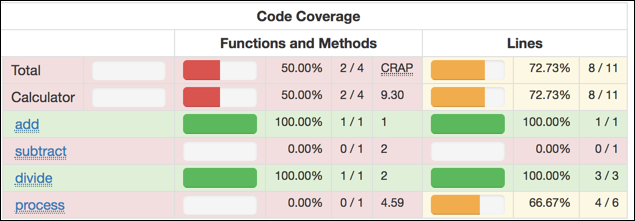
\includegraphics{./tex2pdf.-05a85d9d563be472/093ea6f2954df63fe293cf27e03e06b550d6c326.png}
\caption{Screenshot of HTML coverage report. \label{coverage_html}}
\end{figure}

This is known as code coverage, and easily achieved by:

\begin{enumerate}
\def\labelenumi{\arabic{enumi}.}
\item
  Adding a line to the PHPUnit configuration file (\texttt{php.ini})
\item
  Ensuring the \textbf{xDebug} PHP debugger is installed and activated
\end{enumerate}

See Appendix \ref{appendix_xdebug} for these stesp.

\hypertarget{generating-code-coverage-html-report}{%
\section{Generating Code Coverage HTML
report}\label{generating-code-coverage-html-report}}

Add the following element as a child to the
\texttt{\textless{}logging\textgreater{}} element in file
\texttt{phpuninit.xml.dist}:

\begin{Shaded}
\begin{Highlighting}[]
        \KeywordTok{<log}\OtherTok{ type=}\StringTok{"coverage-html"}\OtherTok{ target=}\StringTok{"./build/report"}\KeywordTok{/>}
\end{Highlighting}
\end{Shaded}

So the full content of the \texttt{\textless{}logging\textgreater{}}
element is now:

\begin{Shaded}
\begin{Highlighting}[]
    \KeywordTok{<logging>}
        \KeywordTok{<log}\OtherTok{ type=}\StringTok{"coverage-html"}\OtherTok{ target=}\StringTok{"./build/report"}\KeywordTok{/>}
        \KeywordTok{<log}\OtherTok{ type=}\StringTok{"junit"}\OtherTok{ target=}\StringTok{"./build/logfile.xml"}\KeywordTok{/>}
        \KeywordTok{<log}\OtherTok{ type=}\StringTok{"testdox-html"}\OtherTok{ target=}\StringTok{"./build/testdox.html"}\KeywordTok{/>}
        \KeywordTok{<log}\OtherTok{ type=}\StringTok{"testdox-text"}\OtherTok{ target=}\StringTok{"./build/testdox.txt"}\KeywordTok{/>}
        \KeywordTok{<log}\OtherTok{ type=}\StringTok{"tap"}\OtherTok{ target=}\StringTok{"./build/logfile.tap"}\KeywordTok{/>}
    \KeywordTok{</logging>}
\end{Highlighting}
\end{Shaded}

Now when you run \texttt{vendor/bin/simple-phpunit} you'll see a new
directory \texttt{report} inside \texttt{/build}. Open the
\texttt{index.html} file in \texttt{/build/report} and you'll see the
main page of your coverage report. See Figure \ref{build_files}.

\begin{figure}
\centering
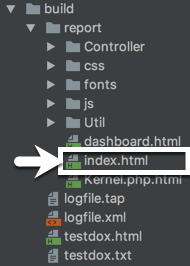
\includegraphics[width=0.75\textwidth,height=\textheight]{./tex2pdf.-05a85d9d563be472/6d9bd18e008151ecb77d2f17729d4c6cfe5c431e.png}
\caption{Build files showing \texttt{index.html} in
\texttt{/build/report}. \label{build_files}}
\end{figure}

\hypertarget{tailoring-the-whitelist}{%
\section{Tailoring the `whitelist'}\label{tailoring-the-whitelist}}

PHPUnit decides which soruces file to analyse and build coverage reports
for by using a `whitelist' - i.e.~a list of just those files and/or
directories that we are interested in at this point in time. The
whitelist is inside the \texttt{\textless{}filter\textgreater{}} element
in PHPUnity configuration file `phpunit.xml.dist'.

the default whitelist is \texttt{./src} - i.e \textbf{all} files in our
source directory. But, for example, this will include Kernel, which we
generally don't touch. So if you want to go \textbf{GREEN} for
everything in your coverage report, then you can list only those
directories inside \texttt{/src} that you are interested in.

For our example above we were working with classes in \texttt{/src/Util}
and \texttt{src/Controller}, so that's what we can list in our
`whitelist'. You can always `disable' lines in XML by wrapping an XML
command around them \texttt{\textless{}-\/-\ ...\ -\/-\textgreater{}},
which we've done below to the default \texttt{./src/} white list
element:

\begin{Shaded}
\begin{Highlighting}[]
    \KeywordTok{<filter>}
        \KeywordTok{<whitelist>}
            \CommentTok{<!--}
\CommentTok{                // ignore this element for now ...}
\CommentTok{                <directory>./src/</directory>}
\CommentTok{            -->}
            \KeywordTok{<directory>}\NormalTok{./src/Controller}\KeywordTok{</directory>}
            \KeywordTok{<directory>}\NormalTok{./src/Util}\KeywordTok{</directory>}
        \KeywordTok{</whitelist>}
    \KeywordTok{</filter>}
\end{Highlighting}
\end{Shaded}

\part{Publishing Symfony websites}

\hypertarget{publishing-your-symfony-website}{%
\chapter{Publishing your Symfony
website}\label{publishing-your-symfony-website}}

\hypertarget{requirements-for-symfony-publishing}{%
\section{Requirements for Symfony
publishing}\label{requirements-for-symfony-publishing}}

You need the following to run Symfony on an internet host:

\begin{itemize}
\item
  an up to date version of PHP (8.1+ at present)
\item
  a MySQL database (or another DB type supported by Symfony)
\item
  a way to setup your project code (e.g.~Composer)
\item
  a way to setup your database (e.g.~SSH terminal to run fixtures or
  MySQL dumps or client connection)
\end{itemize}

Traditional hosting companies, that don't offer SSH terminals, may
require you to use FTP and online MySQL clients (such as PHPMyAdmin) to
setup your project. Once setup, they'll run fine, but there can be a
bunch of fiddly steps with online Control Panels and so on.

Having setup several PHP and Symfony projects for companies and
organisations with traditional hosting companies in the past, I can say
from experience that unless you are doing it every day, it's a fiddly
business, especially when you want to be spending your time adding and
testing features to the website project rather than administering the
site.

\hypertarget{simplest-ways-to-host-symfony-projects}{%
\section{Simplest ways to host Symfony
projects}\label{simplest-ways-to-host-symfony-projects}}

There are 2 easy ways to host Symfony websites, both supporting
\textbf{CD (Continuous Deployment)} whereby commits pushed to the
\textbf{master} branch of a Github (or similar) cloud repository are
pulled down and the app restarted automatically, triggered by web
``hooks'' - event messages to the hosting servers each time a new commit
is pushed:

\begin{itemize}
\item
  Symfony Cloud, from Sensio Labs, the creators of Symfony. See Figure
  \ref{sfCloud}.

  \begin{figure}
  \centering
  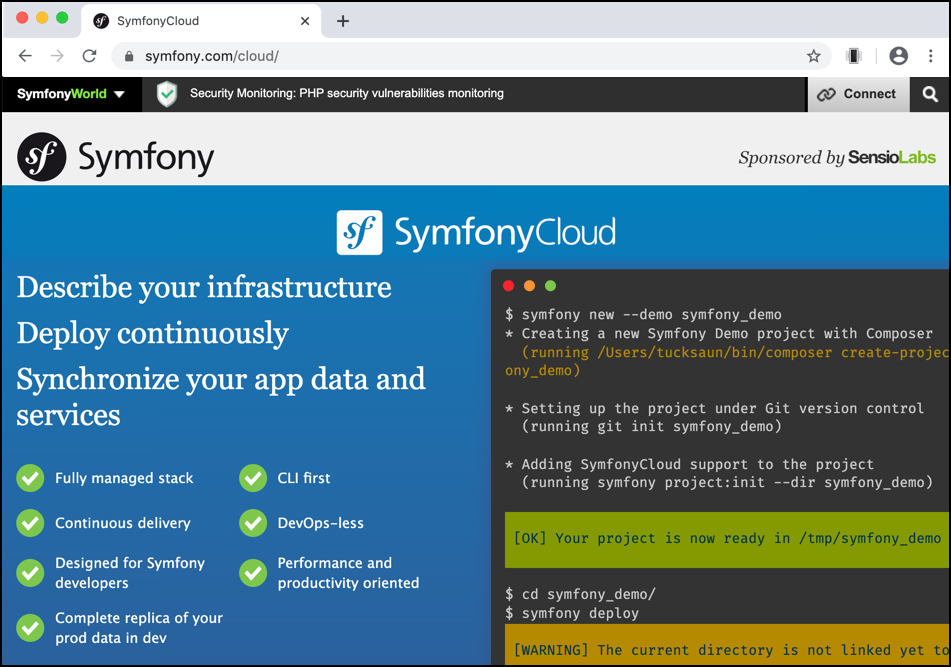
\includegraphics{./tex2pdf.-05a85d9d563be472/e6bbd8d18c9dc496b3cd41bbb14403128085bed7.png}
  \caption{Symfony Cloud - from the creators of Symfony.\label{sfCloud}}
  \end{figure}
\item
  PAAS - PHP-As-A-Service hosting companies

  \begin{itemize}
  \tightlist
  \item
    these companies specialise in PHP projects, and provide PHP
    environment variables, MySQL integrations, Github hooks and so on.
    Fore example see Figure \ref{paas} to see the site for
    \url{Fortrabbit.com}.
  \end{itemize}

  \begin{figure}
  \centering
  
\includegraphics{./tex2pdf.-05a85d9d563be472/705868fe300961a7b7b0974c558cd3a425e1b8ff.png}
  \caption{Fortrabbit.com - PHP-As-A-Service hosting.\label{paas}}
  \end{figure}
\end{itemize}

Since it's cheaper, and still very straightforward, we'll go through the
steps for publishing with \textbf{Fortrabbit}.

\hypertarget{setting-up-project-ready-for-fortrabbit}{%
\chapter{Setting up project ready for
Fortrabbit}\label{setting-up-project-ready-for-fortrabbit}}

\hypertarget{updating-the-names-of-our-mysql-variables-to-match-fortrabbit-ones}{%
\section{Updating the names of our MySQL variables to match Fortrabbit
ones}\label{updating-the-names-of-our-mysql-variables-to-match-fortrabbit-ones}}

By simply changing the names (identifiers) of the variables in our
\texttt{.env} file, it means our application will work locally with
these settings and also work with no further changes when published to
Fortrabbit.

Choose a \textbf{NEW} database name, e.g.~I've chosen
\texttt{week10demo} here. Now edit your project's \texttt{.env} file to
now use variables \texttt{MYSQL\_USER}, \texttt{MYSQL\_PASSWORD},
\texttt{MYSQL\_HOST} and \texttt{MYSQL\_DATABASE} as follows, with
\textbf{your} local root password and new database name:

\begin{verbatim}
    MYSQL_USER=root
    MYSQL_PASSWORD=passpass
    MYSQL_HOST=127.0.0.1:3306
    MYSQL_DATABASE=week10demo
    DATABASE_URL=mysql://${MYSQL_USER}:${MYSQL_PASSWORD}@${MYSQL_HOST}/${MYSQL_DATABASE}
\end{verbatim}

See Figure \ref{mysqlvariables} to see these Fortrabbit MySQL variables
for Symfony project.

\begin{figure}
\centering
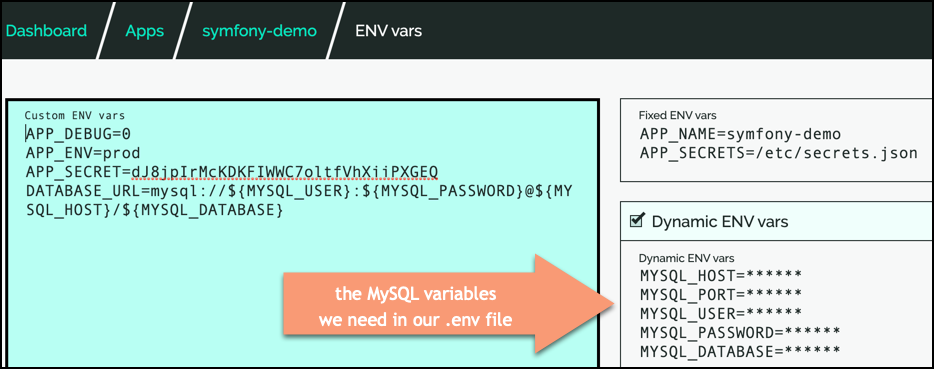
\includegraphics{./tex2pdf.-05a85d9d563be472/05e39c908a0fd75b87cbd978aad52085ca7daf69.png}
\caption{The Fortrabbit MySQL environment
variables.\label{mysqlvariables}}
\end{figure}

\hypertarget{create-new-db-locally-and-make-fresh-migrations}{%
\section{Create new DB locally, and make fresh
migrations}\label{create-new-db-locally-and-make-fresh-migrations}}

Since both locally, and remotely we'll have a new DB, do the following
to keep things in step:

\begin{enumerate}
\def\labelenumi{\arabic{enumi}.}
\item
  Delete any contents in folder \texttt{/migrations} folder (but not the
  folder itself)
\item
  Create the new local database schema with
  \texttt{symfony\ console\ doctrine:database:create}
\item
  Create a migration for this new database with
  \texttt{symfony\ console\ make:migration}
\end{enumerate}

We now have a new clean migration ready to use with our remote database.

\hypertarget{creating-the-public.htaccess-apache-server-routing-file}{%
\section{\texorpdfstring{Creating the \texttt{/public/.htaccess} Apache
server routing
file}{Creating the /public/.htaccess Apache server routing file}}\label{creating-the-public.htaccess-apache-server-routing-file}}

This is a solved problem, since there is a Symfony community Composer
Flex ``recipe'' to copy into our project the file we need.

Type the following a the command line:

\begin{Shaded}
\begin{Highlighting}[]
    \ExtensionTok{composer}\NormalTok{ require symfony/apache-pack}
\end{Highlighting}
\end{Shaded}

You'll be asked to say ``yes'' since this is a community contribution
and not officially part of the Symfony project:

\begin{Shaded}
\begin{Highlighting}[]
\NormalTok{    $ }\ExtensionTok{composer}\NormalTok{ require symfony/apache-pack}

    \ExtensionTok{Using}\NormalTok{ version ^1.0 for symfony/apache-pack}
    \ExtensionTok{./composer.json}\NormalTok{ has been updated}
    \ExtensionTok{Loading}\NormalTok{ composer repositories with package information}
    \ExtensionTok{Updating}\NormalTok{ dependencies (including require-dev)}
    \ExtensionTok{Restricting}\NormalTok{ packages listed in }\StringTok{"symfony/symfony"}\NormalTok{ to }\StringTok{"5.0.*"}
    \ExtensionTok{Package}\NormalTok{ operations: 1 install, 0 updates, 0 removals}
      \ExtensionTok{-}\NormalTok{ Installing symfony/apache-pack (v1.0.1)}\BuiltInTok{:}\NormalTok{ Loading from cache}
    \ExtensionTok{Writing}\NormalTok{ lock file}
    \ExtensionTok{Generating}\NormalTok{ autoload files}
    \ExtensionTok{ocramius}\NormalTok{/package-versions: }\ExtensionTok{Generating}\NormalTok{ version class...}
    \ExtensionTok{ocramius}\NormalTok{/package-versions: }\ExtensionTok{...done}\NormalTok{ generating version class}
    \ExtensionTok{Symfony}\NormalTok{ operations: 1 recipe (b11f4293313a650b4596551c0c2bb403)}
      \ExtensionTok{-}\NormalTok{  WARNING  symfony/apache-pack (}\OperatorTok{>}\NormalTok{=1.0)}\BuiltInTok{:}\NormalTok{ From github.com/symfony/recipes-contrib:master}
        \ExtensionTok{The}\NormalTok{ recipe for this package comes from the }\StringTok{"contrib"}\NormalTok{ repository, which is open to community contributions.}
        \ExtensionTok{Review}\NormalTok{ the recipe at https://github.com/symfony/recipes-contrib/tree/master/symfony/apache-pack/1.0}
    
        \ExtensionTok{Do}\NormalTok{ you want to execute this recipe?}
\NormalTok{        [}\ExtensionTok{y}\NormalTok{] Yes}
\NormalTok{        [}\ExtensionTok{n}\NormalTok{] No}
\NormalTok{        [}\ExtensionTok{a}\NormalTok{] Yes for all packages, only for the current installation session}
\NormalTok{        [}\ExtensionTok{p}\NormalTok{] Yes permanently, never ask again for this project}
        \KeywordTok{(}\ExtensionTok{defaults}\NormalTok{ to n}\KeywordTok{)}\BuiltInTok{:}\NormalTok{ y}
\end{Highlighting}
\end{Shaded}

Say ``y'' here!

\begin{Shaded}
\begin{Highlighting}[]
      \ExtensionTok{-}\NormalTok{ Configuring symfony/apache-pack (}\OperatorTok{>}\NormalTok{=1.0)}\BuiltInTok{:}\NormalTok{ From github.com/symfony/recipes-contrib:master}
    \ExtensionTok{Executing}\NormalTok{ script cache:clear [OK]}
    \ExtensionTok{Executing}\NormalTok{ script assets:install public [OK]}
    
    \ExtensionTok{Some}\NormalTok{ files may have been created or updated to configure your new packages.}
    \ExtensionTok{Please}\NormalTok{ review, edit and commit them: these files are yours.}
\end{Highlighting}
\end{Shaded}

You should then see a new file \texttt{.htaccess} in the
\texttt{/public} folder. See Figure \ref{htaccess}.

\begin{figure}
\centering
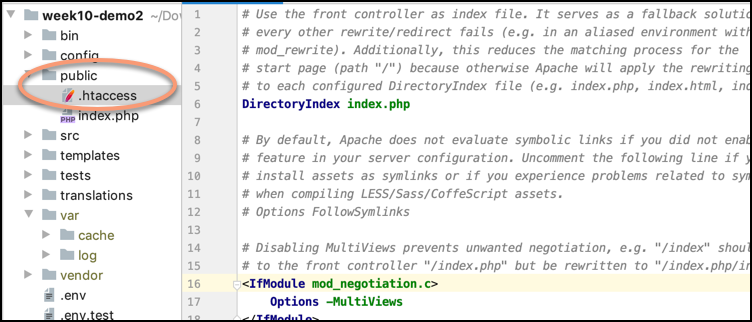
\includegraphics{./tex2pdf.-05a85d9d563be472/e64fef28d6b71f1e73a309396ae3ee2eb5bc20d6.png}
\caption{Screenshot of recipe-created \texttt{/public/.htaccess}
file.\label{htaccess}}
\end{figure}

That's it - we've now prepared our local Symfony project for publishing
at Fortrabbit!

\hypertarget{publishing-with-fortrabbit.com}{%
\chapter{Publishing with
Fortrabbit.com}\label{publishing-with-fortrabbit.com}}

\hypertarget{main-steps-for-paas-publishing-with-fortrabbit}{%
\section{Main steps for PAAS publishing with
Fortrabbit}\label{main-steps-for-paas-publishing-with-fortrabbit}}

Having setup our Symfony project (with \texttt{.htaccess} and renamed
\texttt{.env} MySQL variables and a fresh DB migration), we need to be
able to the following to get our Symfony project published with
Fortrabbit:

\begin{itemize}
\item
  create a Fortrabbit account, and setup SSH security keys so our local
  computer can securely communicate with the Fortrabbit servers

  \begin{itemize}
  \item
    follow the steps in the
    \href{https://help.fortrabbit.com/ssh-keys}{Fortrabbit SHH keys
    documentation}
  \item
    see Figure \ref{sshkeys}
  \end{itemize}
\end{itemize}

\begin{figure}
\centering
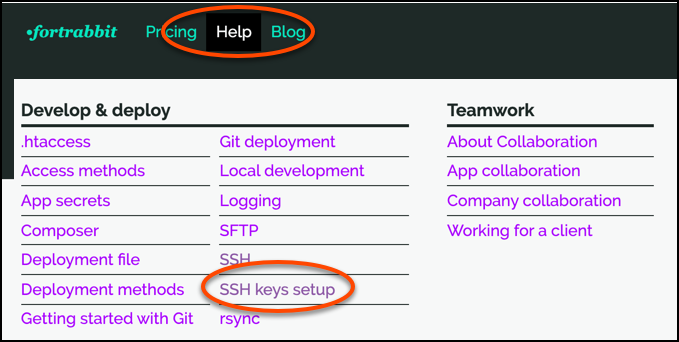
\includegraphics{./tex2pdf.-05a85d9d563be472/ef93043ab1d729cc5f00cf1ca9d77bff502203ac.png}
\caption{Fortrabbit ssh setup documentation.\label{sshkeys}}
\end{figure}

\begin{itemize}
\item
  link a local project to a Fortrabbit Github repository (seee steps in
  next section)

  \begin{itemize}
  \tightlist
  \item
    so we can \textbf{push} our code to the Fortrabbit repo to trigger a
    rebuild of the project
  \end{itemize}
\item
  work in an SSH terminal to run migrations \& fixtures etc. (see later
  this chapter)
\end{itemize}

\hypertarget{create-a-new-fortrabbit-symfony-project}{%
\section{Create a new Fortrabbit Symfony
project}\label{create-a-new-fortrabbit-symfony-project}}

It's very straightforward to setup a new Symfony project on Fortrabbit:

\begin{enumerate}
\def\labelenumi{\arabic{enumi}.}
\item
  Create a new PHP app in Fortrabbit. See Figure \ref{newProject}.
\item
  Choose Symfony project type. See Figure \ref{sfType}.
\item
  Choose European data centre. See Figure \ref{eu}.
\end{enumerate}

\begin{figure}
\centering
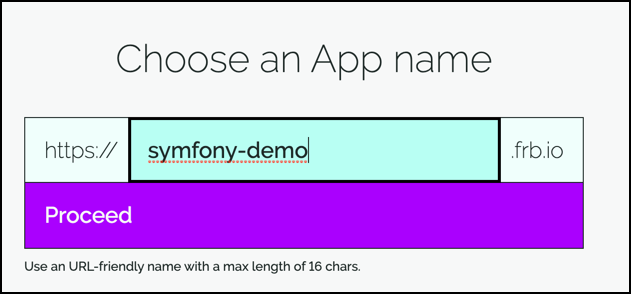
\includegraphics{./tex2pdf.-05a85d9d563be472/9a360b32c70ea3c285bbb50856e2ce22e2df2c33.png}
\caption{Create new app.\label{newProject}}
\end{figure}

\begin{figure}
\centering
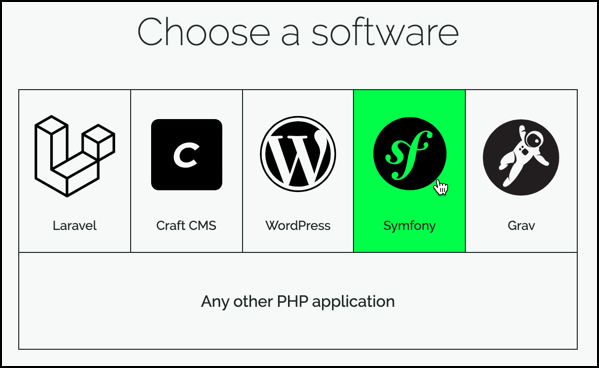
\includegraphics{./tex2pdf.-05a85d9d563be472/cc205075913395d8127679e2a4b238ac9a0e41a3.png}
\caption{Choose Symfony project type.\label{sfType}}
\end{figure}

\begin{figure}
\centering
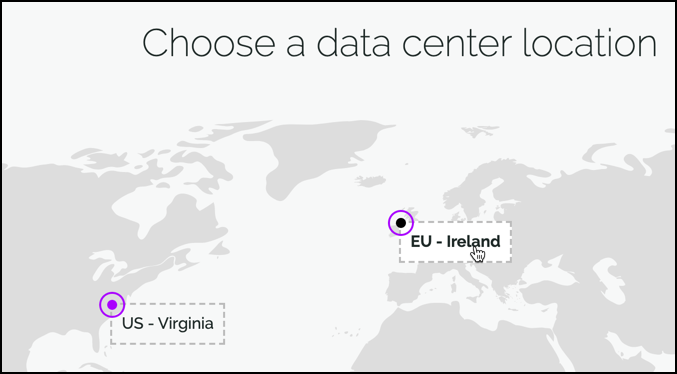
\includegraphics{./tex2pdf.-05a85d9d563be472/d1945750402dc453c6e7ed16c715a6c0c2155740.png}
\caption{Choose EU data centre.\label{eu}}
\end{figure}

\hypertarget{choose-plan---the-trial-is-free}{%
\section{Choose plan - the Trial is
free!}\label{choose-plan---the-trial-is-free}}

There are several plans available. At the time of writing they offered:

\begin{itemize}
\tightlist
\item
  Light at €5 per month
\item
  Standard at €15 per month
\item
  Plus at €30 per month
\end{itemize}

AND there is also a ``free trial'' option - this trial app will be
available for 24-48 hours - long enough for testing \ldots{}

\hypertarget{temporarily-set-project-environment-to-dev-so-we-can-load-db-fixtures}{%
\section{\texorpdfstring{Temporarily set project environment to
\texttt{dev} so we can load DB
fixtures}{Temporarily set project environment to dev so we can load DB fixtures}}\label{temporarily-set-project-environment-to-dev-so-we-can-load-db-fixtures}}

There is an issue in that Fortrabbit sets the Symfony environment as
\texttt{prod}, for production, i.e.~a running live website. This
excludes things like the Symfony profiler, tests and so on. However, it
also stops us from being able to load \textbf{fixtures} via Doctrine.
This makes sense, since we don't want to reset the database for a live
system.

While there are several ways to allow us to load fixtures, the simplest
is to temporarily change the Fortrabbit project to the \texttt{dev}
environnent. We do this by editing the projects \textbf{Custome ENV
variable} \texttt{APP\_ENV} from \texttt{prod} to \texttt{dev}. See
Figures \ref{editEnv} and \ref{devEnvironment}.

\begin{figure}
\centering
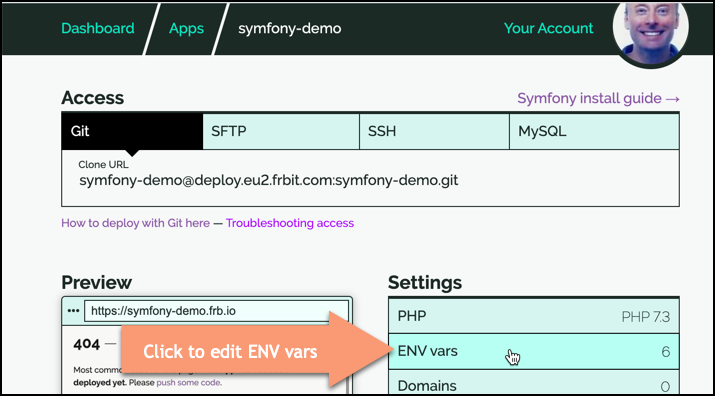
\includegraphics{./tex2pdf.-05a85d9d563be472/95149fc53c4e728e7b82aea00b5ceba9c8bbe42e.png}
\caption{Edit ENV vars for Fortrabbit project.\label{editEnv}}
\end{figure}

\begin{figure}
\centering
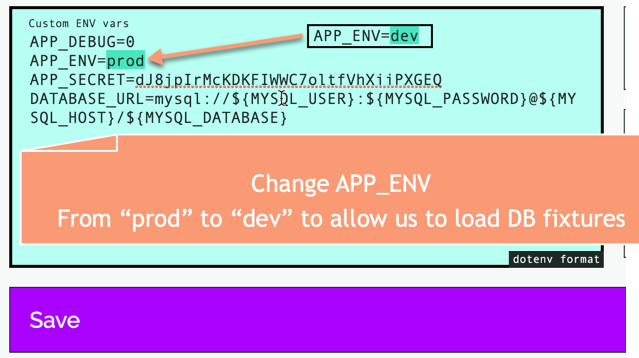
\includegraphics{./tex2pdf.-05a85d9d563be472/894c4dc95e174f508236060fa5116ee86653942c.png}
\caption{Changing environment from \texttt{prod} to \texttt{dev}.
\label{devEnvironment}}
\end{figure}

NOTE: Don't forget to change this back to \texttt{prod} after you have
loaded fixtures \ldots{}

\hypertarget{getting-a-linked-git-project-on-your-local-computer}{%
\section{Getting a linked Git project on your local
computer}\label{getting-a-linked-git-project-on-your-local-computer}}

\begin{enumerate}
\def\labelenumi{\arabic{enumi}.}
\item
  clone the repo to your local machine. See Figure \ref{cloneLocal}.

  \begin{itemize}
  \item
    NOTE: This will be an \textbf{empty} repository folder, apart from
    the hidden \texttt{.git} folder - you'll get a message warning you
    about this when you clone it to your computer
  \item
    you'll copy your project files \textbf{into} this empty folder, to
    push back up to the Fortrabbit repo
  \end{itemize}
\end{enumerate}

\begin{figure}
\centering
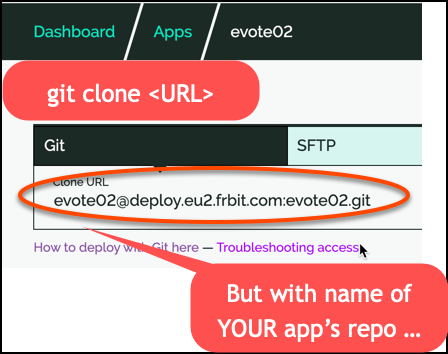
\includegraphics{./tex2pdf.-05a85d9d563be472/c51a23adeab67e7c05dc8b5e9068b31e59612313.png}
\caption{Clone git repo.\label{cloneLocal}}
\end{figure}

\begin{enumerate}
\def\labelenumi{\arabic{enumi}.}
\item
  copy your project files into the newly created cloned project folder
\item
  add all the new files to the current snapshot:

  \texttt{git\ add\ .}
\item
  Create the commit snapshot with a short message (the message doesn't
  matter):

  \texttt{git\ commit\ -m\ "added\ files\ to\ project"}
\item
  Push all these new files and folders up to the Fortrabbit repository:

  \texttt{git\ push}
\end{enumerate}

NOTE: You'll see some Fortrabbit output when it responds to the new
commit to the repositories \texttt{master} branch - CD (Contiuous
Deployment) in action:

\begin{Shaded}
\begin{Highlighting}[]
\NormalTok{    $ }\FunctionTok{git}\NormalTok{ push}
        \ExtensionTok{Enumerating}\NormalTok{ objects: 92, done.}
        \ExtensionTok{Counting}\NormalTok{ objects: 100% (92/92), }\KeywordTok{done}\ExtensionTok{.}
        \ExtensionTok{Delta}\NormalTok{ compression using up to 12 threads}
        \ExtensionTok{Compressing}\NormalTok{ objects: 100% (81/81), }\KeywordTok{done}\ExtensionTok{.}
        \ExtensionTok{Writing}\NormalTok{ objects: 100% (92/92), }\ExtensionTok{49.53}\NormalTok{ KiB }\KeywordTok{|} \ExtensionTok{3.10}\NormalTok{ MiB/s, done.}
        \ExtensionTok{Total}\NormalTok{ 92 (delta 3), }\ExtensionTok{reused}\NormalTok{ 0 (delta 0)}
        
        \ExtensionTok{Commit}\NormalTok{ received, starting build of branch master}
        
\NormalTok{        –––––––––––––––––––––––  ƒ  –––––––––––––––––––––––}
        
        \ExtensionTok{B}\NormalTok{ U I L D}
        \ExtensionTok{Checksum}\NormalTok{:}
          \ExtensionTok{814af6dc566dad405a8d4f13bc990a5e6dda6be7}
        
        \ExtensionTok{Deployment}\NormalTok{ file:}
          \ExtensionTok{not}\NormalTok{ found}
        
        \ExtensionTok{Pre-script}\NormalTok{:}
          \ExtensionTok{not}\NormalTok{ found}
          \ExtensionTok{0ms}
        
        \ExtensionTok{Composer}\NormalTok{:}
          \ExtensionTok{-}\NormalTok{ - -}
          \ExtensionTok{Loading}\NormalTok{ composer repositories with package information}
          \ExtensionTok{Installing}\NormalTok{ dependencies (including require-dev) }\ExtensionTok{from}\NormalTok{ lock file}
          \ExtensionTok{Package}\NormalTok{ operations: 109 installs, 0 updates, 0 removals}
            \ExtensionTok{-}\NormalTok{ Installing ocramius/package-versions (1.5.1)}\BuiltInTok{:}\NormalTok{ Downloading (100%)}
            \ExtensionTok{-}\NormalTok{ Installing symfony/flex (v1.6.2)}\BuiltInTok{:}\NormalTok{ Downloading (100%)}
          
          \ExtensionTok{Prefetching}\NormalTok{ 107 packages }
            \ExtensionTok{-}\NormalTok{ Downloading (100%)}
          
            \ExtensionTok{-}\NormalTok{ Installing doctrine/lexer (1.2.0)}\BuiltInTok{:}\NormalTok{ Loading from cache}
            \ExtensionTok{...}\NormalTok{ lots of installing for the first push ...}
            \ExtensionTok{.............................................}
          
          \ExtensionTok{Executing}\NormalTok{ script cache:clear [OK]}
          \ExtensionTok{Executing}\NormalTok{ script assets:install public [OK]}
          \ExtensionTok{-}\NormalTok{ - -}
          \ExtensionTok{10s}\NormalTok{ 839ms}
        
        \ExtensionTok{Post-script}\NormalTok{:}
          \ExtensionTok{not}\NormalTok{ found}
          \ExtensionTok{0ms}
        
        \ExtensionTok{R}\NormalTok{ E L E A S E}
        
        \ExtensionTok{Packaging}\NormalTok{:}
          \ExtensionTok{3s}\NormalTok{ 796ms}
        
        \ExtensionTok{Revision}\NormalTok{:}
          \ExtensionTok{1585658858201186125.814af6dc566dad405a8d4f13bc990a5e6dda6be7}
        
        \ExtensionTok{Size}\NormalTok{:}
          \ExtensionTok{6.9}\NormalTok{ MB}
        
        \ExtensionTok{Uploading}\NormalTok{:}
          \ExtensionTok{217ms}
        
        \ExtensionTok{Build} \KeywordTok{&} \ExtensionTok{release}\NormalTok{ done in 14s 863ms, now queued for final distribution.}
        
\NormalTok{        –––––––––––––––––––––––  ƒ  –––––––––––––––––––––––}
        
        \ExtensionTok{To}\NormalTok{ deploy.eu2.frbit.com:symfony-demo.git}
         \ExtensionTok{*}\NormalTok{ [new branch]      master -}\OperatorTok{>}\NormalTok{ master }
\end{Highlighting}
\end{Shaded}

\hypertarget{visit-site-to-see-if-published-although-may-be-db-errors}{%
\section{Visit site to see if published (although may be DB
errors)}\label{visit-site-to-see-if-published-although-may-be-db-errors}}

Now visit your website - via link at Fortrabbit. See Figure
\ref{visitSite}.

\begin{itemize}
\tightlist
\item
  NOTE: Since the database isn't setup yet, you'll get an error if your
  homepage tries to list any DB data
\end{itemize}

\begin{figure}
\centering
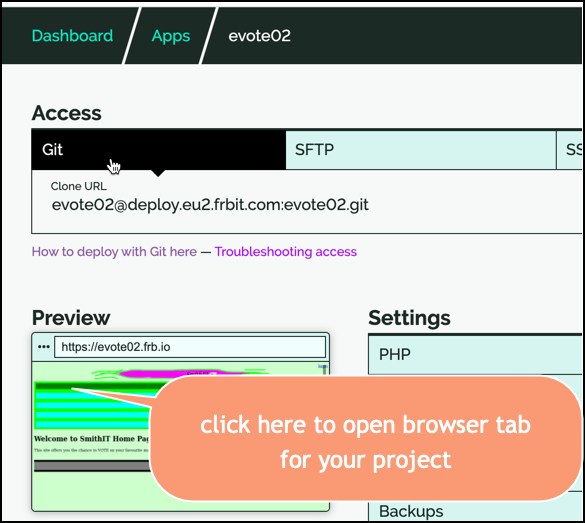
\includegraphics{./tex2pdf.-05a85d9d563be472/b6677ac4cdd6663d8e7aa9970a8c909576cb7ccf.png}
\caption{Visit published website link.\label{visitSite}}
\end{figure}

\hypertarget{connect-command-line-terminal-to-fortrabbit-project-via-shh}{%
\section{Connect command-line terminal to Fortrabbit project via
SHH}\label{connect-command-line-terminal-to-fortrabbit-project-via-shh}}

Via an SSH terminal we can run the migration and load fixtures for our
Fortrabbit app. Note, the database has already been created for us, so
don't try to run a \texttt{database:create} Doctrine command \ldots{}

Use the provided SSH connection command to connect to Fortrabbvit projet
in a terminal. See Figure \ref{sshconnect}.

\begin{figure}
\centering
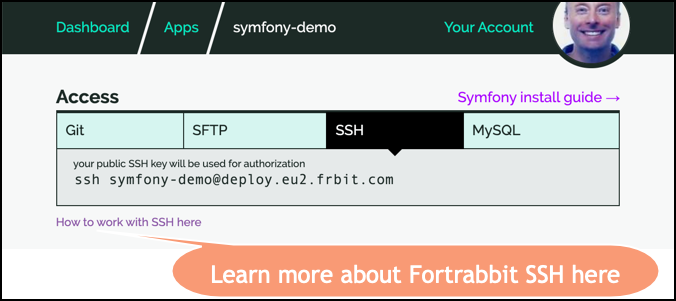
\includegraphics{./tex2pdf.-05a85d9d563be472/c5fe2271f72c3814d3318dbf96eab9df6e3bba6a.png}
\caption{SSH connect command.\label{sshconnect}}
\end{figure}

\hypertarget{use-ssh-to-run-db-migrations}{%
\section{Use SSH to run DB
migrations}\label{use-ssh-to-run-db-migrations}}

We can now run the migration command
\texttt{doctrine:migrations:migrate}. See Figure \ref{migration}.

\begin{figure}
\centering
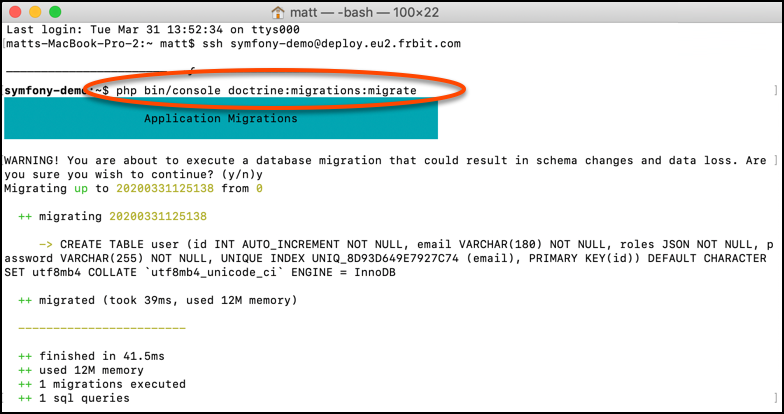
\includegraphics{./tex2pdf.-05a85d9d563be472/c2b9594315902f1538b5476f7dcdadde08c45625.png}
\caption{Running migration in SSH terminal.\label{migration}}
\end{figure}

\hypertarget{use-ssh-to-load-fixtures}{%
\section{Use SSH to load fixtures}\label{use-ssh-to-load-fixtures}}

We can now run the migration command \texttt{doctrine:fixtures:load}.
See Figure \ref{fixtures}.

\begin{figure}
\centering
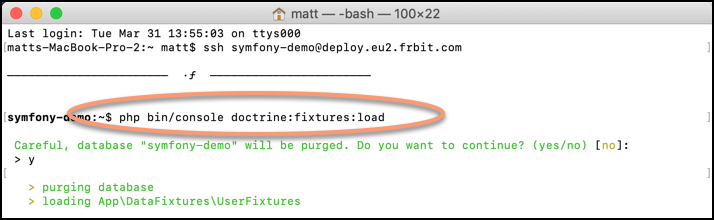
\includegraphics{./tex2pdf.-05a85d9d563be472/74477eb1b4659cc22af3a87e087fdb5f95f2e36c.png}
\caption{Loading fixtures in SSH terminal.\label{fixtures}}
\end{figure}

NOTE: - if you change fixtures, you'll need to repeat this after pushing
the updated code to the Fortrabbit repo

\begin{itemize}
\tightlist
\item
  don't forget to change the project environment back to \texttt{prod}
  if you want a secure, efficient running web application
\end{itemize}

\hypertarget{use-ssh-to-clear-the-symfony-cache}{%
\section{Use SSH to clear the Symfony
cache}\label{use-ssh-to-clear-the-symfony-cache}}

It's a good idea to CLEAR the CACHE after making changes to your
project.

Connected through SSH in the terminal and run the cache clear command:

\begin{Shaded}
\begin{Highlighting}[]
    \ExtensionTok{php}\NormalTok{ bin/console cache:clear}
\end{Highlighting}
\end{Shaded}

\hypertarget{use-doctrine-query-to-check-db-contents}{%
\section{Use Doctrine query to check DB
contents}\label{use-doctrine-query-to-check-db-contents}}

We can use the Doctrine
\texttt{doctrine:query:sql\ "\textless{}SQL\textgreater{}"} command in
an SSH terminal to check the contents of the database. See Figure
\ref{doctrineSQL}.

\begin{figure}
\centering
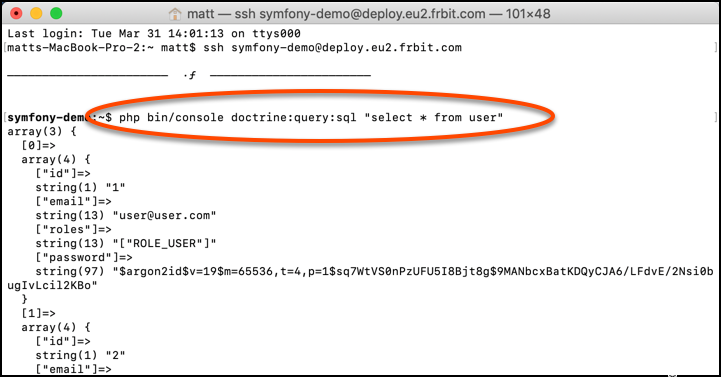
\includegraphics{./tex2pdf.-05a85d9d563be472/dfe7b0b301508f2b683938710f230112e1bcfb93.png}
\caption{SSH terminal running SQL query via
\texttt{doctrine:query:sql}.\label{doctrineSQL}}
\end{figure}

\hypertarget{mysql-queries-using-ssh-tunnel}{%
\section{MySQL queries using SSH tunnel
\ldots{}}\label{mysql-queries-using-ssh-tunnel}}

You can use an SSH tunnel to use your local MySQL terminal to connect to
and query the remote Fortrabbit database

\begin{itemize}
\tightlist
\item
  follow the MySQL help steps from the Fortrabbit App dashboard
\end{itemize}

\begin{figure}
\centering
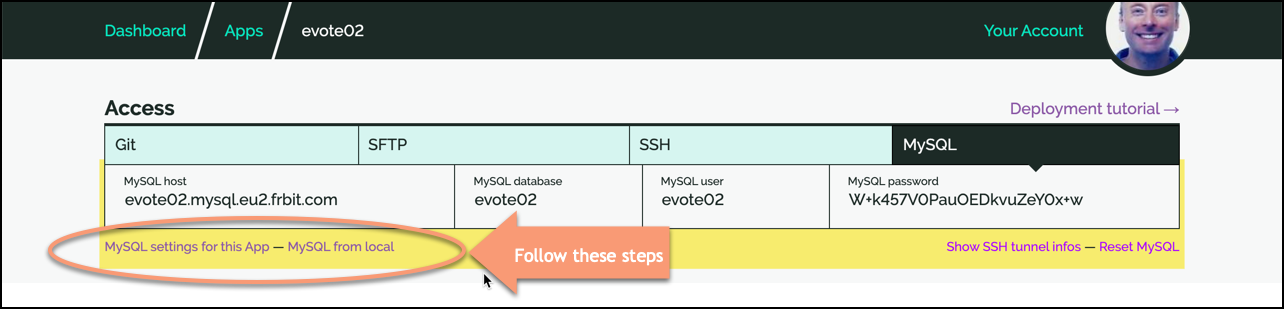
\includegraphics{./tex2pdf.-05a85d9d563be472/a165c9dd7a746479c0c71da7102bdb2b6f5748ea.png}
\caption{Fortrabbt MySQL help.}
\end{figure}

\begin{figure}
\centering
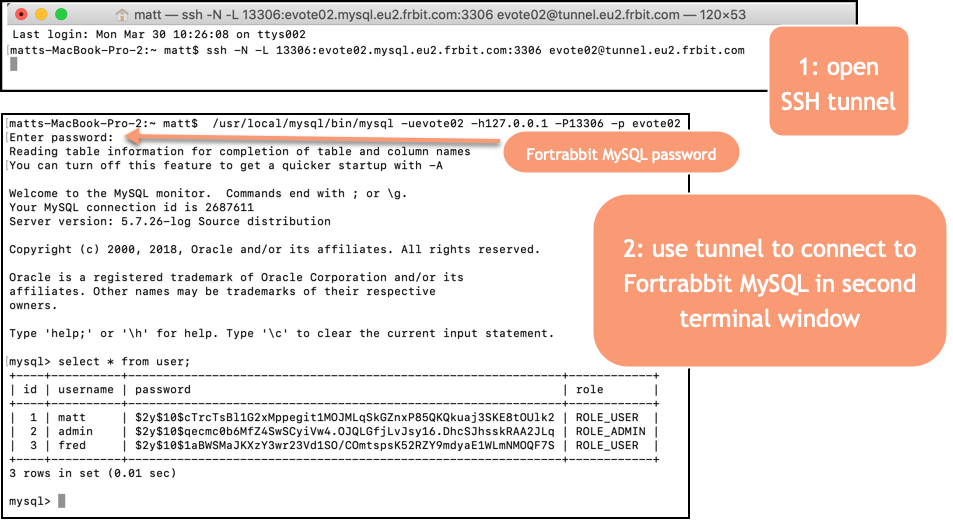
\includegraphics{./tex2pdf.-05a85d9d563be472/4a831ca76089eb2616508f4c80b41db0ca4d5969.png}
\caption{Remote SSH MySQL terminal connection.}
\end{figure}

\hypertarget{published-website}{%
\section{Published website}\label{published-website}}

If all has gone well, you should now have a live published Symfony
website.

NOTE: If you can see the Symfony profiler debug footer, then you've
forgotton to change the envrionment back to \texttt{prod} !!!!

\begin{figure}
\centering
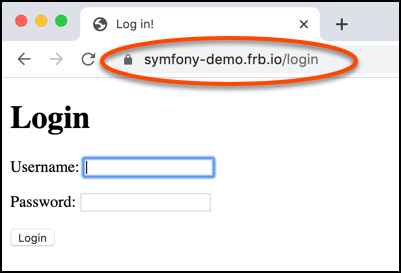
\includegraphics{./tex2pdf.-05a85d9d563be472/5239b2fa165edca2271d5022397983741a2d25bb.png}
\caption{Screenshot of published website.}
\end{figure}

\backmatter

\hypertarget{list-of-references}{%
\chapter{List of References}\label{list-of-references}}

\end{document}
